% =============================================================================
%  Open MCEconomic API --- protocol specification
%
%  Build:  pdflatex OPEN_MCECONOMIC_API_SPECIFICATION.tex   (run twice for the table of contents)
%          or: latexmk -pdf OPEN_MCECONOMIC_API_SPECIFICATION.tex
%
%  Uses only widely-available LaTeX2e packages; no manual installs required.
%  The authoritative source of this content is docs/OPEN_MCECONOMIC_API_SPECIFICATION.md --- keep
%  the two in sync when the protocol changes.
% =============================================================================
\documentclass[11pt,a4paper]{article}

\usepackage[T1]{fontenc}
\usepackage[utf8]{inputenc}
\usepackage{lmodern}
\usepackage{amssymb}
\usepackage{microtype}
\usepackage[margin=2.4cm,headheight=15pt]{geometry}
\usepackage{tikz}
\usetikzlibrary{positioning,arrows.meta,fit,backgrounds,calc,shapes.misc}
\usepackage{xcolor}
\usepackage{titlesec}
\usepackage{fancyhdr}
\usepackage{booktabs}
\usepackage{longtable}
\usepackage{array}
\usepackage{tabularx}
\usepackage{enumitem}
\usepackage{listings}
\usepackage{parskip}
\usepackage[hidelinks]{hyperref}

% ------------------------------------------------------------------ palette --
\definecolor{omceInk}{HTML}{16232B}
\definecolor{omceAccent}{HTML}{0F6E6E}
\definecolor{omceAccentDark}{HTML}{0A4D4D}
\definecolor{omceRule}{HTML}{C9D6D6}
\definecolor{omceWash}{HTML}{F2F7F7}
\definecolor{omceWarnWash}{HTML}{FDF3E7}
\definecolor{omceWarnEdge}{HTML}{C77B2A}
\definecolor{omceCodeBg}{HTML}{F7F9FA}
\definecolor{omceString}{HTML}{9A3A2E}
\definecolor{omceKey}{HTML}{0F6E6E}
\definecolor{omceNum}{HTML}{2F5C9E}
\definecolor{omceMuted}{HTML}{5C6B72}

\color{omceInk}
\hypersetup{
  colorlinks=true, linkcolor=omceAccentDark, urlcolor=omceAccentDark,
  pdftitle={Open MCEconomic API --- Protocol Specification},
  pdfsubject={Remote authoritative economy protocol for Minecraft servers}
}

% ------------------------------------------------------------------ headings --
\titleformat{\section}
  {\normalfont\Large\bfseries\color{omceAccentDark}}{\thesection}{0.7em}{}
  [\vspace{-0.55em}{\color{omceRule}\rule{\linewidth}{0.6pt}}]
\titleformat{\subsection}
  {\normalfont\large\bfseries\color{omceInk}}{\thesubsection}{0.6em}{}
\titleformat{\subsubsection}
  {\normalfont\normalsize\bfseries\color{omceAccentDark}}{\thesubsubsection}{0.6em}{}
\titlespacing*{\section}{0pt}{1.6em}{0.7em}

\pagestyle{fancy}
\fancyhf{}
\renewcommand{\headrulewidth}{0.4pt}
\renewcommand{\headrule}{\hbox to\headwidth{\color{omceRule}\leaders\hrule height \headrulewidth\hfill}}
\fancyhead[L]{\small\color{omceMuted}Open MCEconomic API}
\fancyhead[R]{\small\color{omceMuted}Protocol version 1.0}
\fancyfoot[C]{\small\color{omceMuted}\thepage}

% -------------------------------------------------------------------- macros --
\newcommand{\code}[1]{\texttt{\small #1}}
\newcommand{\req}{\textbf{MUST}}
\newcommand{\rec}{\textbf{SHOULD}}
\newcommand{\opt}{\textbf{MAY}}
\newcommand{\core}{{\small\color{omceAccentDark}\textbf{[core]}}}
\newcommand{\optional}{{\small\color{omceMuted}\textbf{[optional]}}}

% Callout boxes, hand-rolled so the document needs no extra packages.
\newenvironment{callout}[1][omceWash]
  {\par\vspace{0.6em}\noindent
   \begin{tabular}{@{}p{0.3em}@{\hspace{0.7em}}p{\dimexpr\linewidth-2.2em\relax}@{}}
   \cellcolor{#1}\rule{0.3em}{0pt} &
   \begingroup\small}
  {\endgroup\end{tabular}\par\vspace{0.6em}}

\newcommand{\keybox}[2]{%
  \par\vspace{0.5em}\noindent
  \colorbox{#1}{%
    \begin{minipage}{\dimexpr\linewidth-2\fboxsep\relax}
    \vspace{0.35em}\small #2\vspace{0.35em}
    \end{minipage}}%
  \par\vspace{0.5em}}

\newcommand{\note}[1]{\keybox{omceWash}{#1}}
\newcommand{\warn}[1]{\keybox{omceWarnWash}{#1}}

\setlist[itemize]{leftmargin=1.3em,itemsep=0.15em,topsep=0.35em}
\setlist[enumerate]{leftmargin=1.6em,itemsep=0.15em,topsep=0.35em}

\newcolumntype{L}[1]{>{\raggedright\arraybackslash}p{#1}}
\renewcommand{\arraystretch}{1.25}

% ------------------------------------------------------------------ listings --
\lstdefinelanguage{json}{
  showstringspaces=false,
  breaklines=true,
  breakatwhitespace=true,
  literate=
   *{0}{{{\color{omceNum}0}}}{1}{1}{{{\color{omceNum}1}}}{1}
    {2}{{{\color{omceNum}2}}}{1}{3}{{{\color{omceNum}3}}}{1}
    {4}{{{\color{omceNum}4}}}{1}{5}{{{\color{omceNum}5}}}{1}
    {6}{{{\color{omceNum}6}}}{1}{7}{{{\color{omceNum}7}}}{1}
    {8}{{{\color{omceNum}8}}}{1}{9}{{{\color{omceNum}9}}}{1}
    {:}{{{\color{omceInk}{:}}}}{1}
    {,}{{{\color{omceInk}{,}}}}{1}
    {\{}{{{\color{omceAccentDark}{\{}}}}{1}
    {\}}{{{\color{omceAccentDark}{\}}}}}{1}
    {[}{{{\color{omceAccentDark}{[}}}}{1}
    {]}{{{\color{omceAccentDark}{]}}}}{1},
}
\lstset{
  basicstyle=\ttfamily\footnotesize\color{omceInk},
  stringstyle=\color{omceString},
  backgroundcolor=\color{omceCodeBg},
  frame=leftline,
  framerule=1.6pt,
  rulecolor=\color{omceRule},
  framesep=7pt,
  xleftmargin=10pt,
  aboveskip=0.9em,
  belowskip=0.9em,
  columns=fullflexible,
  keepspaces=true,
}
\lstdefinestyle{http}{language=,basicstyle=\ttfamily\footnotesize\color{omceAccentDark}}

% ------------------------------------------------------------------- diagrams --
\tikzset{
  mcbox/.style     = {rounded corners=2pt, draw=omceRule, line width=0.9pt,
                      fill=white, align=center, inner sep=7pt, font=\small},
  authbox/.style   = {rounded corners=2pt, draw=omceAccent, line width=1.3pt,
                      fill=omceWash, align=center, inner sep=7pt, font=\small},
  procbox/.style   = {rounded corners=3pt, draw=omceMuted, line width=0.8pt,
                      dash pattern=on 3pt off 2pt, inner sep=11pt},
  link/.style      = {-{Stealth[length=2.4mm]}, line width=0.9pt, draw=omceInk},
  biglink/.style   = {{Stealth[length=2.4mm]}-{Stealth[length=2.4mm]},
                      line width=1.2pt, draw=omceAccent},
  deadlink/.style  = {-{Stealth[length=2.4mm]}, line width=1.0pt,
                      draw=omceWarnEdge, dash pattern=on 3pt off 2pt},
  lbl/.style       = {font=\scriptsize, align=center, text=omceMuted,
                      inner sep=2pt, fill=white},
  note/.style      = {font=\scriptsize\itshape, align=center, text=omceMuted},
}
\newcommand{\nope}{{\color{omceWarnEdge}\bfseries\large$\times$}}

% =============================================================================
\begin{document}

% ---------------------------------------------------------------- title page --
\begin{titlepage}
\centering
\vspace*{3.2cm}
{\color{omceRule}\rule{\linewidth}{1.2pt}}\\[1.2em]
{\Huge\bfseries\color{omceAccentDark} Open MCEconomic API\par}
\vspace{0.9em}
{\Large\color{omceInk} A remote authoritative economy protocol\\for Minecraft servers\par}
\vspace{0.8em}
{\color{omceRule}\rule{\linewidth}{1.2pt}}\\[2.6em]

\begin{tabular}{r@{\hspace{1.2em}}l}
\color{omceMuted}Protocol version & \textbf{1.0}\\
\color{omceMuted}Status           & Specification\\
\color{omceMuted}Reference client & SUM (Server Utility Mod)\\
\color{omceMuted}Date             & 31 July 2026\\
\end{tabular}

\vspace{3.4cm}
\begin{minipage}{0.82\linewidth}
\small\color{omceMuted}
This document specifies the wire format completely enough that a service can be implemented
against it with no access to any client's source. It is deliberately generic: it describes a
balance-and-ledger service, not any particular product. Any service satisfying the conformance
requirements in Section~\ref{sec:conformance} will interoperate.
\end{minipage}

\vfill
{\small\color{omceMuted}Maintained alongside SUM. Markdown source of record: \code{docs/ECONOMIC\_API.md}}
\end{titlepage}

\tableofcontents
\newpage

% =============================================================================
\section{Overview}

The \textbf{Open MCEconomic API} (OMCE) lets a remote HTTP service act as the authoritative owner
of a Minecraft player economy. The mod is \textbf{always the client}; the remote service is
\textbf{always the authority}. When the API is enabled, the remote service --- not the Minecraft
world save --- is the source of truth for player balances and the permanent transaction ledger.

This specification is maintained alongside \textbf{SUM} (Server Utility Mod), its reference client.
SUM is named throughout as the concrete example of what a client does and needs, but the protocol
itself is vendor-neutral: nothing on the wire is SUM-specific, and any mod or plugin may implement
the client side.

\subsection{Design goals}

\begin{enumerate}
\item \textbf{The remote service is authoritative.} The client never invents money. Every balance it
      shows is a value the service returned, and every change it applies is one the service
      committed.
\item \textbf{Implementable by a modest service.} The required surface is five endpoints.
      Everything else is an advertised capability the client degrades around.
\item \textbf{Safe over an unreliable network.} Minecraft cannot block its tick loop on HTTP. Every
      mutating call is idempotent and independently recoverable, so a timeout never leaves the
      question ``was the player charged twice?'' unanswerable.
\item \textbf{Exactly representable amounts.} Money never crosses the wire as a floating-point
      number.
\item \textbf{Forward-compatible.} Clients add economy features regularly. A service written
      against this document must not need a code change when the client adds a new kind of
      transaction.
\end{enumerate}

\subsection{Terminology}

The key words \req, \textbf{MUST NOT}, \rec, \textbf{SHOULD NOT}, and \opt{} are used as in
RFC~2119.

\begin{tabularx}{\linewidth}{L{3.1cm} X}
\toprule
\textbf{Term} & \textbf{Meaning}\\
\midrule
Service        & The remote HTTP implementation of this API. The authority.\\
Client         & The mod, running on a Minecraft server.\\
Instance       & One Minecraft server talking to the service. Several instances \opt{} share one service.\\
Account        & A settled balance held by the service, identified by an opaque \code{accountId}.\\
Party          & One side of a transaction. May be an account, or a virtual counterparty.\\
Settled party  & A party whose balance the service actually maintains.\\
Virtual party  & A party the service records for audit but holds no balance for.\\
Minor unit     & The smallest indivisible amount of the currency (e.g.\ a cent).\\
\bottomrule
\end{tabularx}

% =============================================================================
\section{Authority model}

A Minecraft economy is larger than ``a number per player''. Some of it stays local. This section is
normative because it tells a service implementer what they are \emph{not} responsible for.

\subsection{Owned by the service}
\begin{itemize}
\item \textbf{Player balances.} The single authoritative number per player.
\item \textbf{The transaction ledger.} A permanent, ordered, auditable record of every movement.
\item \textbf{Policy.} Overdraft rules, spending limits, cooldowns, account freezes.
\item \textbf{Currency definition.} Code, symbol, and scale.
\end{itemize}

\subsection{Owned by the client (the instance)}
\begin{itemize}
\item \textbf{Physical cash.} Bill items are inventory items in the world. The service never sees
      them; it only sees the balance side of an ATM deposit or withdrawal.
\item \textbf{Shop escrow.} A shop block accumulates its takings locally until the owner withdraws.
\item \textbf{Job escrow.} A job listing holds its reward locally between posting and payout.
\item \textbf{Prices.} Shop prices, plot prices, and job rewards are set in-game and stored in-game.
\item \textbf{In-world authority.} Block ownership, permissions, and command access.
\end{itemize}

\subsection{Consequence}

Only \code{player} parties need to be settled. A shop, a job listing, a plot, or a pile of cash is a
\textbf{virtual party}: the service records it as the counterparty on a ledger entry so the books
read correctly, but holds no balance for it. A service \opt{} settle other party types (see
\code{settledPartyTypes} in Section~\ref{sec:health}), but \textbf{MUST NOT} be required to.

\note{This keeps money conserved end to end. A shop purchase debits the buyer against a virtual
\code{shop} party; the later payout credits the owner \emph{from} that same virtual \code{shop}
party. Net effect across the two transactions: buyer down, owner up, nothing created.}

% =============================================================================
\section{Deployment topology}
\label{sec:topology}

Minecraft has two distinct notions of ``client'' and ``server'', and conflating them is the easiest
way to build this wrong. This section fixes exactly which process opens a connection to the
service.

\subsection{The rule}

\warn{\textbf{Only the logical server ever contacts the economy service. A Minecraft client never
does.}}

SUM's balances are already server-authoritative. Every mutation happens in a server-side packet
handler, command, or tile entity; the resulting balance is pushed to the player's Minecraft client
over SUM's own sync packet, and client-side GUIs (wallet HUD, ATM screen, shop GUI, phone app) read
that \textbf{read-only local mirror}. No GUI has ever read a balance from anywhere but the mirror.

The remote backend slots in underneath that existing arrangement: it replaces where the
\emph{server} gets its authoritative number. The client-facing half of the system does not change
at all, and gains no network dependency.

\begin{figure}[h]
\centering
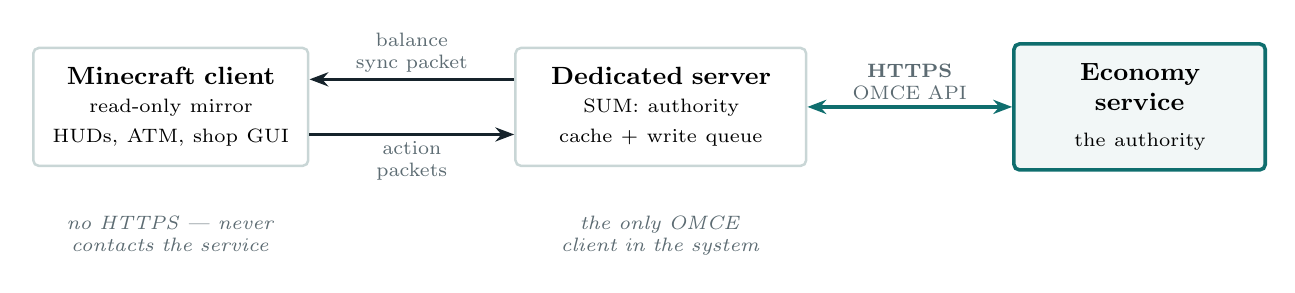
\begin{tikzpicture}[node distance=16mm]
  \node[mcbox, text width=30mm] (client)
    {\textbf{Minecraft client}\\[2pt]
     \scriptsize read-only mirror\\\scriptsize HUDs, ATM, shop GUI};
  \node[mcbox, text width=32mm, right=26mm of client] (server)
    {\textbf{Dedicated server}\\[2pt]
     \scriptsize SUM: authority\\\scriptsize cache + write queue};
  \node[authbox, text width=27mm, right=26mm of server] (service)
    {\textbf{Economy service}\\[2pt]\scriptsize the authority};

  \draw[link] ([yshift=3.5mm]server.west) -- ([yshift=3.5mm]client.east)
        node[lbl, midway, above]{balance\\sync packet};
  \draw[link] ([yshift=-3.5mm]client.east) -- ([yshift=-3.5mm]server.west)
        node[lbl, midway, below]{action\\packets};
  \draw[biglink] (server) -- (service)
        node[lbl, midway, above]{\textbf{HTTPS}\\OMCE API};

  \node[note, below=5mm of client, text width=34mm]
    {no HTTPS --- never contacts the service};
  \node[note, below=5mm of server, text width=36mm]
    {the only OMCE client in the system};
\end{tikzpicture}
\end{figure}

\note{\textbf{Why this matters for the protocol:} the service only ever sees connections from a
small, known set of Minecraft servers --- not from hundreds of player machines. That is what makes
a single shared bearer token per instance reasonable, and why rate limits can be modest.}

\subsection{Why a client must never hold the token}
\label{sec:notoken}

A Minecraft client cannot be trusted with economy credentials:

\begin{itemize}
\item Anything shipped to a client is readable by the player who runs it. A token in a modpack's
      config is a published token.
\item A client that could call \code{/processTransaction} directly could mint itself money, since
      the service has no way to tell a real client from a modified one.
\end{itemize}

\warn{\textbf{Operational warning.} Modpack configs are distributed to players. Do \emph{not} put
\code{authToken}, \code{hmacSecret}, or \code{certificatePassword} in a config that ships with your
pack. The client has no use for them --- it never opens a connection --- so leaving them blank
client-side costs nothing.}

\subsection{The four scenarios}

\begin{tabularx}{\linewidth}{L{5.4cm} L{5.0cm} X}
\toprule
\textbf{Scenario} & \textbf{Who runs the authority} & \textbf{Contacts the service?}\\
\midrule
Dedicated server                    & The server                        & \textbf{Yes} --- the intended deployment\\
Client connected to a server        & Nobody (client mirrors the server) & \textbf{No}\\
Single-player world                 & The \emph{integrated server} inside the game client & \textbf{No}, by default\\
LAN world (``Open to LAN'')         & The integrated server of the host  & \textbf{No}, by default\\
\bottomrule
\end{tabularx}

\subsection{Single-player and the integrated server}
\label{sec:integrated}

This is the case that needs an explicit guard, and it is worth stating plainly:

\warn{\textbf{In Minecraft, single-player is not client-only.} Opening a single-player world starts
a full \emph{integrated server} inside the game client process. All the server-side code --- packet
handlers, commands, capabilities --- runs normally. From SUM's point of view it is a server.}

So a player who has a production config on their machine and opens a single-player world would,
without a guard, connect to the shared economy service and spend real balances from a local save.
SUM therefore gates the remote backend on the server being \textbf{dedicated}:

\begin{lstlisting}[style=http]
if (server != null && configUsable
        && (server.isDedicatedServer() || allowIntegratedServer)) {
    // construct the remote backend
}
\end{lstlisting}

\code{allowIntegratedServer} defaults to \textbf{false}. With it off, a single-player or LAN world
never contacts the service whatever else is in the config, and falls back to the local economy
backends --- so the economy still works, as a separate local economy belonging to that save.

\begin{figure}[h]
\centering
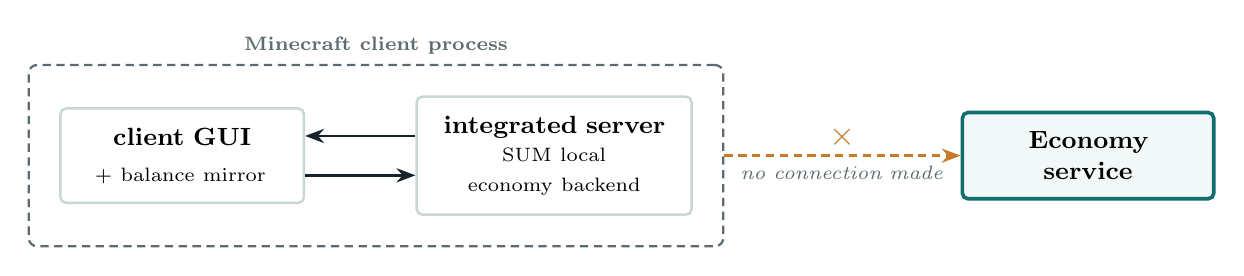
\begin{tikzpicture}[node distance=14mm]
  \node[mcbox, text width=26mm] (gui)
    {\textbf{client GUI}\\[2pt]\scriptsize + balance mirror};
  \node[mcbox, text width=30mm, right=14mm of gui] (int)
    {\textbf{integrated server}\\[2pt]\scriptsize SUM local\\\scriptsize economy backend};
  \draw[link] ([yshift=2.5mm]int.west) -- ([yshift=2.5mm]gui.east);
  \draw[link] ([yshift=-2.5mm]gui.east) -- ([yshift=-2.5mm]int.west);

  \begin{scope}[on background layer]
    \node[procbox, fit=(gui)(int), label={[font=\scriptsize\bfseries, text=omceMuted]above:%
      Minecraft client process}] (proc) {};
  \end{scope}

  \node[authbox, text width=27mm, right=34mm of int] (service)
    {\textbf{Economy service}};
  \draw[deadlink] (proc.east) -- node[lbl, midway, above]{\nope}
        node[note, midway, below, text width=30mm]{no connection made} (service.west);
\end{tikzpicture}
\end{figure}

Set \code{allowIntegratedServer} to \code{true} only if you deliberately want a single-player world
to transact against the live economy --- for instance an administrator testing the integration
locally. Even then, the request still reports itself as \code{integrated} via
\code{X-MCE-Environment} (Section~\ref{sec:reqheaders}), so the service can apply its own policy.

\subsection{Multiple servers, one economy}

Several Minecraft servers \opt{} share one service. Each is a distinct \textbf{instance} and sends
its own \code{X-MCE-Instance} header, which the service records on every ledger entry so activity
can be attributed per server.

Instances do not coordinate with each other. Because the service is the single authority and every
balance carries a \code{version} (Section~\ref{sec:getbalances}), a player who earns money on one
server sees it on another as soon as that server's next balance refresh or \code{/getEvents} poll
lands.

\begin{figure}[h]
\centering
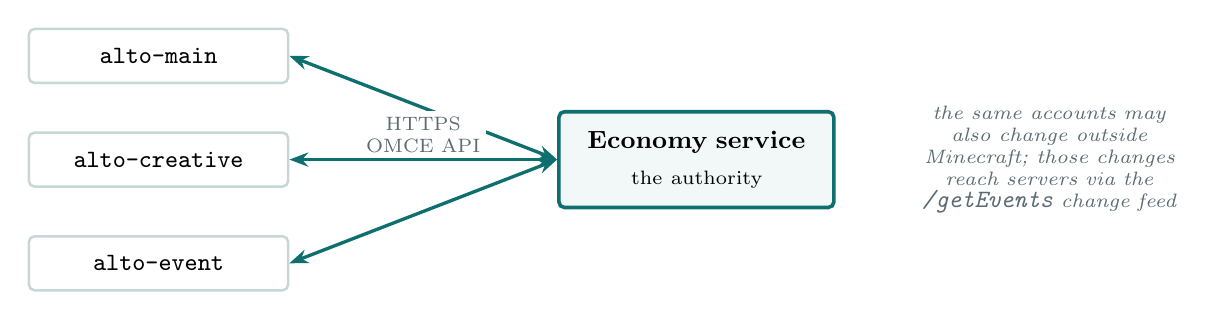
\begin{tikzpicture}[node distance=6mm]
  \node[mcbox, text width=28mm] (s1) {\code{alto-main}};
  \node[mcbox, text width=28mm, below=of s1] (s2) {\code{alto-creative}};
  \node[mcbox, text width=28mm, below=of s2] (s3) {\code{alto-event}};
  \node[authbox, text width=30mm, right=34mm of s2] (service)
    {\textbf{Economy service}\\[2pt]\scriptsize the authority};

  \draw[biglink] (s1.east) -- (service.west);
  \draw[biglink] (s2.east) -- node[lbl, midway, above]{HTTPS\\OMCE API} (service.east-|service.west);
  \draw[biglink] (s3.east) -- (service.west);

  \node[note, right=8mm of service, text width=36mm, anchor=west]
    {the same accounts may also change outside Minecraft; those changes reach servers via the
     \code{/getEvents} change feed};
\end{tikzpicture}
\end{figure}

Each instance \rec{} hold its own bearer token so a single compromised server can be revoked
without disturbing the others.

% =============================================================================
\section{Transport}

\begin{tabularx}{\linewidth}{L{4.2cm} X}
\toprule
\textbf{Property} & \textbf{Value}\\
\midrule
Protocol            & HTTP/1.1 or HTTP/2\\
Transport security  & \textbf{HTTPS REQUIRED} (Section~\ref{sec:tls})\\
Base path           & \code{<baseUrl>/api/economic/v1}\\
Encoding            & UTF-8\\
Request body        & \code{application/json} on every \code{POST}\\
Response body       & \code{application/json} on \emph{every} response, including errors\\
\bottomrule
\end{tabularx}

\code{<baseUrl>} is configured in the client (Section~\ref{sec:config}) --- e.g.\
\code{https://economy.example.net}, making the transaction endpoint\\
\code{https://economy.example.net/api/economic/v1/processTransaction}. The scheme \req{} be
\code{https} (Section~\ref{sec:tls}).

\subsection{Versioning}

The major version is in the path (\code{/v1}). Within a major version the service \req{} remain
backward-compatible: it \opt{} add response fields and \req{} tolerate unknown request fields, but
\textbf{MUST NOT} remove or repurpose either. A breaking change requires \code{/v2}.

Both sides also exchange a full version string: the client sends
\code{X-MCE-Protocol-Version:~1.0} on every request, and the service returns
\code{protocolVersion} in every response envelope. If the service cannot serve the requested major
version it \req{} reply \code{400} with \code{PROTOCOL\_VERSION\_UNSUPPORTED}.

\subsection{Standard request headers}
\label{sec:reqheaders}

\begin{tabularx}{\linewidth}{L{5.0cm} L{1.9cm} X}
\toprule
\textbf{Header} & \textbf{Required} & \textbf{Description}\\
\midrule
\code{Authorization}           & Yes        & \code{Bearer <token>}\\
\code{Content-Type}            & On POST    & \code{application/json; charset=utf-8}\\
\code{Accept}                  & Yes        & \code{application/json}\\
\code{X-MCE-Protocol-Version}  & Yes        & \code{1.0}\\
\code{X-MCE-Instance}          & Yes        & Instance identifier, e.g.\ \code{alto-main}\\
\code{X-MCE-Environment}       & Yes        & \code{dedicated} or \code{integrated}; see below\\
\code{X-MCE-Request-Id}        & Yes        & A fresh UUIDv4 per HTTP attempt; log correlation only\\
\code{Idempotency-Key}         & On mutating calls & See Section~\ref{sec:idempotency}\\
\code{X-MCE-Timestamp}         & If HMAC enabled & Unix milliseconds\\
\code{X-MCE-Signature}         & If HMAC enabled & Hex HMAC-SHA256\\
\code{User-Agent}              & Yes        & \code{<client>/<version> OpenMCEconomicAPI/1.0}\\
\bottomrule
\end{tabularx}

\note{\textbf{\code{X-MCE-Request-Id} vs \code{Idempotency-Key}:} the request id changes on every
retry; the idempotency key does not. The service keys deduplication off the idempotency key
\emph{only}.}

\subsubsection*{\code{X-MCE-Environment}}

Declares what kind of Minecraft server is calling, \textbf{regardless of any client-side setting}:

\begin{tabularx}{\linewidth}{L{3.0cm} X}
\toprule
\textbf{Value} & \textbf{Meaning}\\
\midrule
\code{dedicated}  & A standalone Minecraft server process. The normal production case\\
\code{integrated} & A server running inside a game client --- a single-player or LAN world
                    (Section~\ref{sec:integrated})\\
\bottomrule
\end{tabularx}

The client \req{} send this truthfully on \emph{every} request, deriving it from the actual runtime
environment and never from configuration. A client reaching the service from a single-player world
(because its operator set \code{allowIntegratedServer}) still reports \code{integrated}.

This exists so the service can enforce its own policy rather than trusting the client's. A service
\opt{} \textbf{reject} \code{integrated} requests outright with \code{403} /
\code{ENVIRONMENT\_REJECTED}, \textbf{accept but flag} them by recording the environment on the
ledger entry, or \textbf{ignore} the header entirely --- the default for a service that does not
care. A service that rejects \code{integrated} traffic \rec{} do so at \code{/health} as well, so
the client discovers it at startup and degrades cleanly rather than failing on a player's first
purchase.

% -----------------------------------------------------------------------------
\subsection{Optional integrity headers}
\label{sec:integrity}

These carry context about the calling Minecraft server that a service can use for anomaly detection
and strict policy. SUM sends them by default; they can be disabled with
\code{sendIntegrityHeaders}.

A service \req{} function correctly when they are absent --- \textbf{unless it explicitly
declares them required}. A service \opt{} require any of them and reject requests that omit
them, provided it publishes that policy via \code{requiredHeaders} in \code{/health} and
\code{/getRequiredHeaders} (Section~\ref{sec:reqheaderspolicy}), and rejects with
\code{MISSING\_REQUIRED\_HEADER}. Requiring a header without publishing it is non-conforming:
a client cannot guess.

\begin{tabularx}{\linewidth}{L{4.6cm} L{2.0cm} X}
\toprule
\textbf{Header} & \textbf{Example} & \textbf{What it tells the service}\\
\midrule
\code{X-MCE-Online-Mode}     & \code{true}         & Whether the server authenticates players against Mojang\\
\code{X-MCE-World-Id}        & \code{9c1f\ldots}   & Stable UUID for the world save, persisted in it\\
\code{X-MCE-World-Seq}       & \code{48211}        & Monotonic counter in the world save, incremented per transaction\\
\code{X-MCE-Session-Id}      & \code{4a2b\ldots}   & UUID regenerated on every server boot\\
\code{X-MCE-Player-Count}    & \code{14}           & Players online at the time of the request\\
\code{X-MCE-Initiator-State} & \code{creative,op}  & Risk-relevant state of the initiating player\\
\code{X-MCE-Mod-Version}     & \code{2026.07.31}   & Version of the mod acting as client\\
\bottomrule
\end{tabularx}

\subsubsection*{\code{X-MCE-Online-Mode} --- the one that matters most}

\warn{A Minecraft server running with \code{online-mode=false} does \textbf{not} authenticate
players. Anyone can join using any username and receive that username's UUID. On such a server the
Minecraft UUID in a request is an unverified claim, and the identity model of
Section~\ref{sec:identity} does not hold.}

A service \rec{} refuse or heavily restrict traffic from an offline-mode server, because it cannot
meaningfully attribute a balance to a person. This is the most valuable of these headers: it is a
genuine statement about whether identity means anything, not a heuristic. Services that accept
offline-mode traffic \rec{} at minimum record it on every ledger entry.

\subsubsection*{\code{X-MCE-World-Id} and \code{X-MCE-World-Seq} --- rollback detection}

This pair is the only one with real teeth, because it is a \textbf{consistency check against the
service's own records} rather than a claim the service must take on faith.

\code{X-MCE-World-Seq} is a counter stored \emph{in the world save} and incremented on every
transaction sent. The service remembers the highest value seen per \code{X-MCE-World-Id}. Under
normal operation it only climbs. If a server restores a world backup, the save reverts --- and so
does the counter, so the service sees a sequence number at or below one it has already recorded.

\note{That signature matters because a rolled-back world is the classic Minecraft economy
duplication exploit: the world's local state (shop escrow, job listings, items, chest contents)
returns to an earlier point while the service's ledger does not. Everything spent in the rolled-back
window has been effectively refunded in-world while remaining credited in the ledger.}

A service detecting a regression \rec{} alert an operator and \opt{} refuse writes from that world
until an administrator acknowledges it. It \textbf{SHOULD NOT} silently reject, since a legitimate
restore after hardware failure produces exactly the same signal and needs a human decision.
\code{X-MCE-Session-Id} distinguishes a restart (new session, counter continues) from a rollback
(new session, counter regresses), which is what makes the two separable.

\subsubsection*{\code{X-MCE-Initiator-State}}

A comma-separated list, empty when nothing applies: \code{creative}, \code{spectator}, \code{op},
\code{cheats}, \code{singleplayer}.

\code{creative} is the notable one: a player in creative mode can spawn items and blocks freely, so
selling goods to a shop or an admin-run buy station is effectively minting money. A service \opt{}
reject transactions carrying \code{creative}, or record them for review.

\subsubsection*{What is deliberately not sent}

These headers are intended to be \textbf{cheap, non-invasive, and relevant to the transaction at
hand}. They describe the \emph{economic trustworthiness of the environment}, not the people in it.
The following are excluded from this specification, and a conforming client \textbf{MUST NOT} send
them:

\begin{itemize}
\item Player IP addresses, hostnames, or any network identifiers.
\item Hardware, machine, or installation fingerprints.
\item The server's own address, MOTD, or port.
\item The roster of online players, or any player identity other than the parties to the
      transaction.
\item The installed mod list, or hashes of it.
\item The world seed, or world contents.
\end{itemize}

A service \textbf{MUST NOT} require any of these as a condition of service. If a stricter policy is
needed than these headers support, the correct control is the token: issue it only to server
operators you are willing to trust.

\subsubsection*{What these headers are not}

\warn{\textbf{These are self-reported and therefore not a security boundary.} A modified client can
send whatever it likes. They exist so an \emph{honest} client can tell the service something useful,
and so an \emph{inconsistent} one becomes visible --- not to stop a dishonest one.

The real boundary is the bearer token, which never leaves the server operator's hands
(Section~\ref{sec:notoken}). If you do not trust the operator of a Minecraft server, do not issue
them a token; no header will compensate.

The exception is the \code{X-MCE-World-Seq} check, which has value precisely because the service
validates it against its own ledger rather than believing it.}

\subsection{Standard response headers}

\begin{tabularx}{\linewidth}{L{5.0cm} L{1.9cm} X}
\toprule
\textbf{Header} & \textbf{Required} & \textbf{Description}\\
\midrule
\code{Content-Type}           & Yes & \code{application/json; charset=utf-8}\\
\code{X-MCE-Protocol-Version} & Yes & The version actually served\\
\code{Retry-After}            & On \code{429}/\code{503} & Seconds, or an HTTP-date\\
\code{Deprecation}            & No  & RFC 8594; set when the endpoint or version is deprecated\\
\code{Sunset}                 & No  & RFC 8594 HTTP-date after which it stops working\\
\bottomrule
\end{tabularx}

% =============================================================================
\section{Authentication and security}

\subsection{Bearer token (required)}

Every request carries \code{Authorization: Bearer <token>}. The token is a shared secret issued by
the service operator and configured in the client. Tokens \rec{} be per-instance so one compromised
Minecraft server can be revoked without disturbing others.

A missing, malformed, or unknown token \req{} produce \code{401} with \code{UNAUTHENTICATED}. A
valid token without permission for the requested operation \req{} produce \code{403} with
\code{FORBIDDEN}. The token \textbf{MUST NOT} appear in service logs or in any response body.

\subsection{HMAC request signing (optional)}
\label{sec:hmac}

When the operator enables signing, the client additionally sends \code{X-MCE-Timestamp} and
\code{X-MCE-Signature}. The signature is computed as:

\begin{lstlisting}[style=http]
signingString = METHOD + "\n"
              + PATH_WITH_QUERY + "\n"
              + X-MCE-Timestamp + "\n"
              + SHA256_HEX(rawRequestBody)      // SHA256_HEX("") for GET

X-MCE-Signature = HEX(HMAC_SHA256(sharedSecret, signingString))
\end{lstlisting}

\code{rawRequestBody} is the exact bytes sent --- the service \req{} verify against the raw body,
not a re-serialization of the parsed JSON.

The service \req{} reject a failing signature (\code{401} / \code{SIGNATURE\_INVALID}) and \rec{}
reject a timestamp outside a $\pm$300 second window (\code{401} /
\code{TIMESTAMP\_OUT\_OF\_RANGE}). The comparison \req{} be constant-time. Signing is an
\emph{addition} to the bearer token, never a replacement.

\subsection{Authorization scope}

Administrative commands call the same endpoints as ordinary gameplay. A service \rec{} distinguish
them: the client marks such requests with \code{"initiator": \{"role": "admin", \ldots\}}, and the
service \opt{} require an elevated token for them, replying \code{403} / \code{FORBIDDEN}
otherwise.

\subsection{Transport security}
\label{sec:tls}

\warn{\textbf{HTTPS is REQUIRED.} Every request carries a bearer token in a header, and every
response carries account balances; over plaintext both are readable and forgeable by anything on
the network path.}

\subsubsection*{Service requirements}
\begin{itemize}
\item The service \req{} serve the API over TLS. TLS 1.2 is the minimum; TLS 1.3 \rec{} be
      preferred.
\item The service \rec{} redirect or reject plaintext requests rather than serving them. A client
      \textbf{MUST NOT} follow a redirect that downgrades \code{https} to \code{http}.
\end{itemize}

\subsubsection*{Client requirements}
\begin{itemize}
\item The client \req{} reject a \code{baseUrl} whose scheme is not \code{https}, refusing to start
      the economy backend and logging the reason, unless the operator has explicitly set
      \code{enableHttp}.
\item \code{enableHttp} defaults to \textbf{false} and exists only for local development against a
      service on \code{localhost}. When enabled, the client \req{} log a prominent warning on
      \emph{every} server startup, not just the first.
\item The client \req{} verify the certificate chain \emph{and} the hostname by default. There is
      no ``disable verification'' switch --- self-signed and private-CA deployments are supported
      by supplying the certificate instead.
\end{itemize}

\subsubsection*{Self-signed and private-CA certificates}

Operators running their own certificate authority, or a self-signed certificate, configure
\code{certificatePath} rather than disabling verification. The value is a path \textbf{relative to
the client's config file} (absolute paths are also accepted), pointing at the certificate or CA
bundle to trust.

\begin{tabularx}{\linewidth}{L{3.0cm} L{4.0cm} X}
\toprule
\textbf{Format} & \textbf{Extensions} & \textbf{Notes}\\
\midrule
PEM      & \code{.pem}, \code{.crt}, \code{.cer} & Preferred. One or more \code{BEGIN CERTIFICATE} blocks.\\
PKCS\#12 & \code{.p12}, \code{.pfx}              & Requires \code{certificatePassword}.\\
Java KeyStore & \code{.jks}                      & Requires \code{certificatePassword}.\\
\bottomrule
\end{tabularx}

When \code{certificatePath} is set, the client builds a trust store containing the platform's
default trust anchors \textbf{plus} the supplied certificate(s), so a private CA can be added
without losing the ability to verify public ones. Hostname verification still applies. An
unreadable, malformed, or expired certificate is a fatal configuration error --- the client refuses
to enable the economy backend rather than silently falling back to an unverified connection.

\subsection{Other requirements}
\begin{itemize}
\item The service \rec{} rate limit per token.
\item The service \textbf{MUST NOT} trust any economic claim in a request beyond the parties,
      amount, and type --- in particular it \req{} independently validate balance sufficiency. A
      balance echoed by the client is a cache read, never an assertion.
\item The service \req{} treat player-supplied strings (\code{playerName}, \code{reason},
      \code{metadata} values) as untrusted text.
\end{itemize}

% =============================================================================
\section{Common conventions}

\subsection{Response envelope}

\emph{Every} response --- success or failure, every endpoint --- is a JSON object with at least:

\begin{lstlisting}[language=json]
{
  "ok": true,
  "protocolVersion": "1.0",
  "requestId": "5c9f2a1e-9d1b-4a3f-8a7e-2d5f0b1c3e44",
  "serverTime": "2026-07-31T18:22:04.117Z"
}
\end{lstlisting}

\begin{tabularx}{\linewidth}{L{3.2cm} L{1.9cm} L{1.9cm} X}
\toprule
\textbf{Field} & \textbf{Type} & \textbf{Required} & \textbf{Description}\\
\midrule
\code{ok}              & boolean & Yes & \code{true} on success, \code{false} on failure\\
\code{protocolVersion} & string  & Yes & Version served\\
\code{requestId}       & string  & Yes & Echo of \code{X-MCE-Request-Id}, or service-generated\\
\code{serverTime}      & string  & Yes & RFC 3339 UTC timestamp with milliseconds\\
\code{error}           & object  & When \code{ok=false} & See Section~\ref{sec:errors}\\
\bottomrule
\end{tabularx}

Endpoint-specific fields sit alongside these at the top level. A failure response \textbf{MUST NOT}
carry endpoint payload fields, with the single documented exception in
Section~\ref{sec:processtransaction}.

\subsection{Money representation}
\label{sec:money}

\warn{\textbf{Money MUST NOT cross the wire as a floating-point number.} Every amount in this API
is a JSON \textbf{integer} count of \textbf{minor units}.}

The service declares its scale once, in \code{/health}:

\begin{lstlisting}[language=json]
"currency": {
  "code": "SUM",
  "symbol": "$",
  "minorUnitDigits": 2,
  "displayName": "Dollars"
}
\end{lstlisting}

\code{minorUnitDigits} is the power of ten between a minor unit and a whole unit:

\begin{tabularx}{\linewidth}{L{3.6cm} L{4.2cm} X}
\toprule
\code{minorUnitDigits} & \textbf{1 whole unit =} & \code{amount: 12500} \textbf{means}\\
\midrule
\code{2} & 100 minor units  & \$125.00\\
\code{0} & 1 minor unit     & \$12,500\\
\code{3} & 1000 minor units & \$12.500\\
\bottomrule
\end{tabularx}

\subsubsection*{Rules}
\begin{itemize}
\item \code{amount} is always a \textbf{non-negative} integer. Direction is expressed by
      \code{source} and \code{destination}, never by the sign of \code{amount}.
\item Amounts and balances \req{} fit in a signed 64-bit integer.
\item The service \req{} reject a non-integer, negative, or out-of-range \code{amount} with
      \code{AMOUNT\_INVALID}.
\item A \code{currency} that is not the service's currency code \req{} be rejected with
      \code{CURRENCY\_MISMATCH}.
\end{itemize}

\subsubsection*{Client-side conversion}

SUM stores balances internally as a double-precision dollar value. At the API boundary it converts:

\begin{lstlisting}[style=http]
amountMinor = round(dollars * 10^minorUnitDigits)     // half-up
dollars     = amountMinor / 10^minorUnitDigits
\end{lstlisting}

When \code{minorUnitDigits} is smaller than the client's in-game precision (most importantly
\code{0}, a whole-unit currency), the client \textbf{rounds every price up to the next
representable unit before charging} and displays the rounded price in-game, so a player is never
quoted a price the service cannot settle.

\subsection{Identity and accounts}
\label{sec:identity}

The client knows players by Minecraft UUID and name. The service is not required to use either as
its primary key --- it may key accounts however it likes. Therefore:

\begin{itemize}
\item The client sends \textbf{Minecraft identity}; the service resolves it to an account.
\item The service returns an \textbf{opaque \code{accountId} string}. The client caches it, echoes
      it back, and never parses it.
\item Player UUIDs are sent canonical, hyphenated, lowercase
      (\code{f84c6a79-0a4e-45e0-879b-cd49ebd4c4e2}).
\item \code{playerName} is advisory. Minecraft names change; UUIDs do not. The service \req{} key
      off the UUID and \rec{} store the most recent name for display.
\end{itemize}

\textbf{Unlinked players.} If a service requires players to link a Minecraft account before
transacting, an unresolved player \req{} produce \code{ACCOUNT\_NOT\_LINKED} --- a distinct code
from \code{UNKNOWN\_ACCOUNT} --- and \rec{} include a human-readable instruction in
\code{error.details.linkInstructions}, which the client relays verbatim into chat.

\textbf{Auto-provisioning.} A service \opt{} create an account on first sight of a UUID, declaring
this with the \code{autoProvisionAccounts} capability.

\subsection{Party objects}
\label{sec:parties}

A \textbf{party} is one side of a transaction.

\begin{lstlisting}[language=json]
{ "type": "player",
  "playerUuid": "f84c6a79-0a4e-45e0-879b-cd49ebd4c4e2",
  "playerName": "SomePlayer",
  "accountId": "acct_10457" }

{ "type": "shop",
  "id": "shop:overworld:120:64:-33",
  "name": "Alex's Emporium",
  "ownerUuid": "f84c6a79-0a4e-45e0-879b-cd49ebd4c4e2" }
\end{lstlisting}

\begin{tabularx}{\linewidth}{L{2.7cm} L{1.7cm} L{2.5cm} X}
\toprule
\textbf{Field} & \textbf{Type} & \textbf{Required} & \textbf{Description}\\
\midrule
\code{type}       & string & Yes                    & Party type; see below\\
\code{playerUuid} & string & For \code{player}      & Canonical Minecraft UUID\\
\code{playerName} & string & No                     & Current name, $\leq$ 32 chars. Advisory\\
\code{accountId}  & string & No                     & Previously resolved opaque id\\
\code{id}         & string & For non-\code{player}  & Stable identifier, $\leq$ 128 chars\\
\code{name}       & string & No                     & Human-readable label, $\leq$ 64 chars\\
\code{ownerUuid}  & string & No                     & Owning player, where one exists. Audit only\\
\bottomrule
\end{tabularx}

\subsubsection*{Reserved party types}

\begin{tabularx}{\linewidth}{L{2.4cm} L{2.4cm} X}
\toprule
\code{type} & \textbf{Settled?} & \textbf{Meaning}\\
\midrule
\code{player}   & \textbf{Always} & A player's account. The only type a service \req{} settle\\
\code{shop}     & Virtual & A player-run shop block. \code{id} encodes world and position\\
\code{job}      & Virtual & A job-board listing holding escrowed reward\\
\code{plot}     & Virtual & A land plot being bought or refunded\\
\code{cash}     & Virtual & Physical bill items in the world; ATM deposits and withdrawals\\
\code{system}   & Virtual & A money sink or faucet inside the client (fees, rewards, grants)\\
\code{external} & Virtual & Something outside the game, for service-originated entries\\
\bottomrule
\end{tabularx}

A service \req{} accept any of these types and \textbf{MUST NOT} reject a transaction merely
because a party type is virtual.

\note{\textbf{Composition rule.} Every transaction \req{} have at least one \code{player} party. Two
\code{player} parties means a transfer between accounts. One \code{player} party means money enters
or leaves the settled economy. \emph{Zero} \code{player} parties \req{} be rejected with
\code{NO\_SETTLED\_PARTY}, unless the service declares the corresponding type in
\code{settledPartyTypes}.}

\subsection{Transactions}
\label{sec:transactions}

A transaction is a single atomic movement of \code{amount} from \code{source} to
\code{destination}.

\textbf{Semantics:} \code{source} \emph{pays}; \code{destination} \emph{receives}. If \code{source}
is a settled account it is debited by \code{amount}. If \code{destination} is a settled account it
is credited by \code{amount} $-$ \code{fee.amount}.

\subsubsection*{Transaction types}

\code{type} is a lowercase \code{snake\_case} string. SUM's current vocabulary:

\begin{tabularx}{\linewidth}{L{4.0cm} L{1.9cm} L{2.1cm} X}
\toprule
\code{type} & \textbf{Source} & \textbf{Destination} & \textbf{Emitted when}\\
\midrule
\code{player\_transfer}  & \code{player} & \code{player} & \code{/pay <player> <amount>}\\
\code{atm\_withdraw}     & \code{player} & \code{cash}   & Player withdraws bills at an ATM\\
\code{atm\_deposit}      & \code{cash}   & \code{player} & Player deposits bills at an ATM\\
\code{shop\_purchase}    & \code{player} & \code{shop}   & Buyer purchases from a shop block\\
\code{shop\_payout}      & \code{shop}   & \code{player} & Owner withdraws accumulated takings\\
\code{job\_post\_escrow} & \code{player} & \code{job}    & Poster funds a job listing\\
\code{job\_payout}       & \code{job}    & \code{player} & Completed job approved\\
\code{job\_refund}       & \code{job}    & \code{player} & Listing cancelled or expired\\
\code{plot\_purchase}    & \code{player} & \code{plot}   & Player buys a plot\\
\code{plot\_refund}      & \code{plot}   & \code{player} & Plot purchase reversed\\
\code{loyalty\_reward}   & \code{system} & \code{player} & Playtime or loyalty milestone\\
\code{admin\_credit}     & \code{system} & \code{player} & Admin grant\\
\code{admin\_debit}      & \code{player} & \code{system} & Admin deduction\\
\code{admin\_migration}  & either        & either        & Bulk migration between backends\\
\bottomrule
\end{tabularx}

\warn{\textbf{Forward compatibility (important).} This vocabulary \emph{will grow}. A service
\textbf{MUST NOT} reject an unrecognised \code{type}. It \req{} record the string verbatim and
settle using the \code{source}/\code{destination} semantics above, which are complete on their own.
A service \opt{} offer a strict mode, but \req{} default to permissive and \req{} declare
strictness via the \code{strictTransactionTypes} capability.}

\subsubsection*{Fees}

A transaction \opt{} carry a fee, deducted from what the destination receives:

\begin{lstlisting}[language=json]
"fee": {
  "amount": 250,
  "destination": { "type": "system", "id": "sink.pay_fee" }
}
\end{lstlisting}

The source is charged the full \code{amount}; the destination receives \code{amount} $-$
\code{fee.amount}; the fee goes to \code{fee.destination}, defaulting to
\code{\{"type": "system", "id": "sink.fee"\}}. \code{fee.amount} \req{} satisfy
$0 \leq \mathit{fee} \leq \mathit{amount}$. A service that does not support fees declares
\code{"fees": false}; the client then splits the movement into two transactions.

\subsubsection*{Initiator}

\begin{lstlisting}[language=json]
"initiator": {
  "playerUuid": "f84c6a79-0a4e-45e0-879b-cd49ebd4c4e2",
  "playerName": "SomePlayer",
  "role": "player"
}
\end{lstlisting}

\code{role} is one of \code{player}, \code{admin}, \code{system}. Used for authorization and audit.

\subsubsection*{Metadata and free text}

\begin{tabularx}{\linewidth}{L{2.4cm} L{6.0cm} X}
\toprule
\textbf{Field} & \textbf{Limit} & \textbf{Notes}\\
\midrule
\code{reason}   & $\leq$ 256 chars & Human-readable one-liner, safe for an audit log\\
\code{metadata} & $\leq$ 16 keys; keys $\leq$ 64, values $\leq$ 256 chars & Flat string$\to$string map\\
\bottomrule
\end{tabularx}

Both are untrusted, player-influenced text. The service \req{} store them safely, \textbf{MUST NOT}
interpret them, and \req{} reject over-limit values with \code{MALFORMED\_REQUEST} rather than
silently truncating.

\subsubsection*{Transaction status}

\begin{tabularx}{\linewidth}{L{2.6cm} X}
\toprule
\code{status} & \textbf{Meaning}\\
\midrule
\code{committed} & Applied and durable. The only status permitting an irreversible in-game side effect\\
\code{pending}   & Accepted but not final. The client \req{} poll \code{/getTransaction} before acting\\
\code{held}      & Funds reserved, not yet captured. Only from \code{/authorizeHold}\\
\code{voided}    & Reversed by \code{/voidTransaction}, or a capture that never happened\\
\code{rejected}  & Not applied. Accompanied by an \code{error}\\
\bottomrule
\end{tabularx}

\subsection{Idempotency}
\label{sec:idempotency}

Minecraft servers time out, retry, and restart. Without idempotency, a timed-out purchase would be
indistinguishable from a failed one and players would be double-charged.

\begin{enumerate}
\item The client \req{} send an \code{Idempotency-Key} header on every mutating request. The value
      is a UUIDv4 generated \textbf{once per logical operation} and reused across every retry.
\item \code{/processTransaction} also carries it in the body as \code{idempotencyKey}. If both are
      present and differ, the service \req{} reject with \code{MALFORMED\_REQUEST}.
\item The service \req{} persist the key with the full response it produced for \textbf{at least 24
      hours}.
\item On a repeat with a \textbf{matching} body, the service \textbf{MUST NOT} apply the operation
      again. It \req{} return the \textbf{original stored response} with
      \code{transaction.replayed} set to \code{true} and the original HTTP status.
\item On a repeat with a \textbf{different} body, the service \req{} reject with \code{409} and
      \code{IDEMPOTENCY\_KEY\_REUSED}, applying nothing.
\item If a request with a known key arrives while the first is still in flight, the service \req{}
      either block until the first completes and return its response, or reply \code{409} with
      \code{IDEMPOTENCY\_IN\_PROGRESS} and \code{retryable: true}.
\end{enumerate}

Body matching \rec{} use a canonical hash of the semantically meaningful fields (type, amount,
currency, parties, fee), not raw bytes --- the client does not guarantee stable JSON key ordering
across retries.

\note{\textbf{Recovery.} If the client never receives a response, it retries with the same key.
Once retries are exhausted it calls \code{GET /getTransaction?idempotencyKey=\ldots} to discover the
true outcome. A service \req{} support that lookup --- it is how every ambiguous outcome is
resolved.}

\subsection{Errors}
\label{sec:errors}

\begin{lstlisting}[language=json]
"error": {
  "code": "INSUFFICIENT_FUNDS",
  "message": "Balance 4200 is below the required 12500.",
  "retryable": false,
  "retryAfterMs": null,
  "details": { "balance": 4200, "required": 12500, "shortfall": 8300 }
}
\end{lstlisting}

\begin{tabularx}{\linewidth}{L{2.7cm} L{1.7cm} L{1.7cm} X}
\toprule
\textbf{Field} & \textbf{Type} & \textbf{Required} & \textbf{Description}\\
\midrule
\code{code}         & string  & Yes & \code{SCREAMING\_SNAKE\_CASE}, from the table below\\
\code{message}      & string  & Yes & English, $\leq$ 512 chars. Diagnostic, not player-facing\\
\code{retryable}    & boolean & Yes & Whether retrying the identical request could succeed\\
\code{retryAfterMs} & integer & No  & Minimum wait before retry\\
\code{details}      & object  & No  & Structured, code-specific context\\
\bottomrule
\end{tabularx}

The client maps codes to player-facing chat text itself; \code{message} goes to the server log. An
unknown \code{code} is treated as \code{INTERNAL\_ERROR} with \code{retryable} honoured as sent.

\subsubsection*{Error code table}

\begin{longtable}{L{5.0cm} L{1.0cm} L{1.6cm} L{6.4cm}}
\toprule
\textbf{Code} & \textbf{HTTP} & \textbf{Retryable} & \textbf{Meaning}\\
\midrule
\endfirsthead
\toprule
\textbf{Code} & \textbf{HTTP} & \textbf{Retryable} & \textbf{Meaning}\\
\midrule
\endhead
\code{UNAUTHENTICATED}               & 401 & No  & Missing or bad bearer token\\
\code{SIGNATURE\_INVALID}            & 401 & No  & HMAC verification failed\\
\code{TIMESTAMP\_OUT\_OF\_RANGE}     & 401 & No  & \code{X-MCE-Timestamp} outside the window\\
\code{FORBIDDEN}                     & 403 & No  & Token lacks permission\\
\code{ENVIRONMENT\_REJECTED}         & 403 & No  & Refused on environment policy; \code{details.reason} names the cause\\
\code{PROTOCOL\_VERSION\_UNSUPPORTED}& 400 & No  & Major version not served\\
\code{MALFORMED\_REQUEST}            & 400 & No  & Bad JSON, missing field, or limit exceeded\\
\code{MISSING\_REQUIRED\_HEADER}     & 400 & No  & A required header is absent or disallowed; \code{details.header} names it\\
\code{AMOUNT\_INVALID}               & 400 & No  & Non-integer, negative, or out-of-range amount\\
\code{CURRENCY\_MISMATCH}            & 400 & No  & Not this service's currency\\
\code{NO\_SETTLED\_PARTY}            & 400 & No  & Neither party is settleable\\
\code{UNSUPPORTED\_PARTY\_TYPE}      & 400 & No  & Party type not recognised (strict services)\\
\code{UNSUPPORTED\_TRANSACTION\_TYPE}& 400 & No  & Type not recognised (strict services)\\
\code{UNKNOWN\_ACCOUNT}              & 404 & No  & No account, and auto-provisioning is off\\
\code{ACCOUNT\_NOT\_LINKED}          & 409 & No  & Player must link their account first\\
\code{ACCOUNT\_FROZEN}               & 409 & No  & Account administratively blocked\\
\code{INSUFFICIENT\_FUNDS}           & 409 & No  & Debit would overdraw\\
\code{LIMIT\_EXCEEDED}               & 409 & Maybe & Policy limit or cooldown; use \code{retryAfterMs}\\
\code{IDEMPOTENCY\_KEY\_REUSED}      & 409 & No  & Key reused with a different body\\
\code{IDEMPOTENCY\_IN\_PROGRESS}     & 409 & \textbf{Yes} & First request with this key still running\\
\code{TRANSACTION\_NOT\_FOUND}       & 404 & No  & No transaction with that id or key\\
\code{NOT\_VOIDABLE}                 & 409 & No  & Too old, or a non-reversible type\\
\code{ALREADY\_VOIDED}               & 409 & No  & Already reversed\\
\code{HOLD\_EXPIRED}                 & 409 & No  & Hold lapsed before capture\\
\code{HOLD\_ALREADY\_SETTLED}        & 409 & No  & Hold already captured or released\\
\code{VERSION\_CONFLICT}             & 409 & No  & \code{expectedVersion} did not match\\
\code{CURSOR\_EXPIRED}               & 410 & No  & Event cursor too old to serve\\
\code{RATE\_LIMITED}                 & 429 & \textbf{Yes} & Too many requests; honour \code{Retry-After}\\
\code{ECONOMY\_READ\_ONLY}           & 503 & \textbf{Yes} & Reads served, writes suspended\\
\code{SERVICE\_UNAVAILABLE}          & 503 & \textbf{Yes} & Temporarily down\\
\code{INTERNAL\_ERROR}               & 500 & \textbf{Yes} & Unexpected failure\\
\bottomrule
\end{longtable}

The HTTP status \req{} agree with the code. The client keys its behaviour off \code{code} and
\code{retryable}, using the status only for coarse logging.

\subsection{Rate limiting}

The service \rec{} rate limit per token, replying \code{429} with \code{RATE\_LIMITED} and a
\code{Retry-After} header. A busy 40-player server generates on the order of a few requests per
second at peak. The client retries \code{429} with exponential backoff and full jitter, honouring
\code{Retry-After} as a floor, and \textbf{MUST NOT} retry a non-retryable error.

% =============================================================================
\section{Endpoints}

\begin{tabularx}{\linewidth}{L{1.6cm} L{5.6cm} X}
\toprule
\textbf{Method} & \textbf{Path} & \textbf{Tier}\\
\midrule
\code{GET}  & \code{/health}             & \core\\
\code{GET}  & \code{/getRequiredHeaders} & \optional{} \code{headerPolicy}\\
\code{POST} & \code{/resolveAccounts}    & \core\\
\code{POST} & \code{/getBalances}        & \core\\
\code{POST} & \code{/processTransaction} & \core\\
\code{POST} & \code{/validateTransaction}& \optional{} \code{preflight}\\
\code{GET}  & \code{/getTransaction}     & \core\\
\code{GET}  & \code{/getBalance}         & \optional{} convenience\\
\code{POST} & \code{/voidTransaction}    & \optional{} \code{void}\\
\code{POST} & \code{/setBalance}         & \optional{} \code{setBalance}\\
\code{POST} & \code{/authorizeHold}      & \optional{} \code{holds}\\
\code{POST} & \code{/captureHold}        & \optional{} \code{holds}\\
\code{POST} & \code{/releaseHold}        & \optional{} \code{holds}\\
\code{GET}  & \code{/getLedger}          & \optional{} \code{ledger}\\
\code{GET}  & \code{/getEvents}          & \optional{} \code{events}\\
\code{GET}  & \code{/getLeaderboard}     & \optional{} \code{leaderboard}\\
\bottomrule
\end{tabularx}

\note{\textbf{Why \code{POST} for some reads?} \code{/getBalances} and \code{/resolveAccounts} take
a list of players. Sixty UUIDs do not belong in a query string, and the client must refresh every
online player in one call. These are POST-with-a-body reads: safe, they change nothing, and they
carry no \code{Idempotency-Key}.}

% -----------------------------------------------------------------------------
\subsection{\code{GET /health} \core}
\label{sec:health}

Liveness and handshake. The client calls this at startup, after any sustained failure, and every
\code{healthPollSeconds}. The response drives every degrade-and-fallback decision.

\textbf{Request:} no body. \code{Authorization} is \textbf{REQUIRED} --- the service \textbf{MUST
NOT} publish capabilities anonymously.

\begin{lstlisting}[language=json]
{
  "ok": true, "protocolVersion": "1.0", "requestId": "...",
  "serverTime": "2026-07-31T18:22:04.117Z",
  "status": "ok",
  "implementation": { "name": "example-economy", "version": "3.2.1" },
  "currency": {
    "code": "SUM", "symbol": "$", "minorUnitDigits": 2, "displayName": "Dollars"
  },
  "capabilities": {
    "void": true, "setBalance": true, "holds": false,
    "preflight": true, "headerPolicy": true,
    "ledger": true, "events": true, "leaderboard": true,
    "fees": true, "negativeBalances": false,
    "autoProvisionAccounts": true, "strictTransactionTypes": false,
    "offlinePlayers": true
  },
  "settledPartyTypes": ["player"],
  "requiredHeaders": ["Authorization", "X-MCE-Instance", "X-MCE-Online-Mode"],
  "limits": {
    "maxBatchAccounts": 100,
    "maxTransactionAmount": 100000000,
    "requestsPerMinute": 600,
    "idempotencyRetentionHours": 72
  }
}
\end{lstlisting}

\begin{tabularx}{\linewidth}{L{3.6cm} L{1.9cm} L{1.7cm} X}
\toprule
\textbf{Field} & \textbf{Type} & \textbf{Required} & \textbf{Description}\\
\midrule
\code{status}            & string   & Yes & \code{ok}, \code{degraded}, or \code{read\_only}\\
\code{implementation}    & object   & No  & Service name and version, for logging\\
\code{currency}          & object   & Yes & See Section~\ref{sec:money}\\
\code{capabilities}      & object   & Yes & Optional-feature flags; absent means \code{false}\\
\code{settledPartyTypes} & string[] & Yes & Types held balances for; \req{} include \code{player}\\
\code{requiredHeaders}   & string[] & Yes & Headers this service rejects requests without; may be empty\\
\code{limits}            & object   & Yes & See below\\
\bottomrule
\end{tabularx}

\begin{tabularx}{\linewidth}{L{5.4cm} X}
\toprule
\code{limits} \textbf{field} & \textbf{Description}\\
\midrule
\code{maxBatchAccounts}          & Max entries per batch call. \req{} be $\geq$ 50\\
\code{maxTransactionAmount}      & Largest single \code{amount} accepted, in minor units\\
\code{requestsPerMinute}         & Advertised rate limit\\
\code{idempotencyRetentionHours} & How long keys are remembered. \req{} be $\geq$ 24\\
\bottomrule
\end{tabularx}

\subsubsection*{Capability fallbacks}

\begin{tabularx}{\linewidth}{L{4.6cm} X}
\toprule
\textbf{Flag} & \textbf{If \code{false}, the client\ldots}\\
\midrule
\code{void}                   & issues a compensating reverse transaction instead\\
\code{preflight}              & answers affordability from its cached balance only\\
\code{headerPolicy}           & relies on the \code{requiredHeaders} summary in \code{/health} alone\\
\code{setBalance}             & reads the balance and computes a delta (with a race warning)\\
\code{holds}                  & debits immediately and reverses on failure\\
\code{ledger}                 & omits in-game transaction history UI\\
\code{events}                 & polls \code{/getBalances} on a timer instead\\
\code{leaderboard}            & omits any economy leaderboard\\
\code{fees}                   & splits fee-bearing transfers into two transactions\\
\code{negativeBalances}       & never sends \code{allowNegative}\\
\code{autoProvisionAccounts}  & treats \code{UNKNOWN\_ACCOUNT} as permanent per player\\
\code{strictTransactionTypes} & (if \emph{true}) warns the operator that new features may break\\
\code{offlinePlayers}         & avoids transacting for players who are not online\\
\bottomrule
\end{tabularx}

\code{status: "read\_only"} tells the client to serve balances from cache and refuse spending with
a clear maintenance message, rather than failing every purchase with a generic error.

% -----------------------------------------------------------------------------
\subsection{\code{GET /getRequiredHeaders} \optional{} \code{headerPolicy}}
\label{sec:reqheaderspolicy}

Publishes the service's header policy: which headers it requires, which it merely uses, and which it
ignores. A client can call this once at startup and know before its first real request whether it is
able to satisfy the service. The same information is summarised in \code{/health} as
\code{requiredHeaders}, so a minimal client never needs this endpoint; it exists for completeness
and for richer, per-endpoint policy.

\begin{lstlisting}[language=json]
{
  "ok": true, "protocolVersion": "1.0", "requestId": "...", "serverTime": "...",
  "headers": [
    { "name": "Authorization", "requirement": "required", "appliesTo": "*",
      "description": "Bearer token issued by the economy operator." },
    { "name": "Idempotency-Key", "requirement": "required",
      "appliesTo": ["/processTransaction", "/voidTransaction", "/setBalance"],
      "description": "UUIDv4, stable across retries of one logical operation." },
    { "name": "X-MCE-Online-Mode", "requirement": "required", "appliesTo": "*",
      "acceptedValues": ["true"],
      "description": "This economy does not accept offline-mode servers." },
    { "name": "X-MCE-World-Seq", "requirement": "recommended",
      "appliesTo": ["/processTransaction"],
      "description": "Used for rollback detection; requests without it are flagged." },
    { "name": "X-MCE-Player-Count", "requirement": "ignored", "appliesTo": "*" }
  ],
  "policyVersion": "2026-07-31"
}
\end{lstlisting}

\begin{tabularx}{\linewidth}{L{4.4cm} L{2.6cm} L{1.6cm} X}
\toprule
\textbf{Field} & \textbf{Type} & \textbf{Required} & \textbf{Description}\\
\midrule
\code{headers}                 & array    & Yes & One entry per header the service has an opinion about\\
\code{headers[].name}          & string   & Yes & Header name, case-insensitive\\
\code{headers[].requirement}   & string   & Yes & \code{required}, \code{recommended}, \code{optional}, or \code{ignored}\\
\code{headers[].appliesTo}     & string \textbar{} string[] & Yes & \code{"*"} for all endpoints, or a list of paths\\
\code{headers[].acceptedValues}& string[]  & No  & If present, the value \req{} be one of these\\
\code{headers[].description}   & string   & No  & Human-readable rationale, for diagnostics\\
\code{policyVersion}           & string   & No  & Opaque version; changes when the policy does\\
\bottomrule
\end{tabularx}

The list is \emph{not} exhaustive of all headers the service tolerates --- anything absent is
treated as \code{optional}. A service \textbf{MUST NOT} list a header as \code{required} that this
specification defines as optional \emph{and} that it does not genuinely enforce; the point of the
endpoint is that a client can trust it.

\subsubsection*{Rejecting requests with missing headers}

A service \opt{} require any header, including the optional integrity headers of
Section~\ref{sec:integrity}. When a required header is missing or carries a disallowed value, it
\req{} reject with \code{400} and \code{MISSING\_REQUIRED\_HEADER}, naming the header:

\begin{lstlisting}[language=json]
{
  "ok": false,
  "error": {
    "code": "MISSING_REQUIRED_HEADER",
    "message": "This economy requires X-MCE-Online-Mode: true.",
    "retryable": false,
    "details": { "header": "X-MCE-Online-Mode", "received": "false",
                 "acceptedValues": ["true"] }
  }
}
\end{lstlisting}

\begin{itemize}
\item The service \req{} apply the same policy to \code{/health}, so a client that cannot satisfy it
      discovers this at startup rather than on a player's first purchase.
\item The service \textbf{MUST NOT} require a header this specification does not define, unless it
      also publishes it here. A client cannot guess.
\item The service \rec{} keep the policy stable. Tightening it takes every existing client offline
      at once.
\end{itemize}

SUM logs the full header policy at startup when \code{verboseLogging} is on, and refuses to enable
the economy backend with a specific operator-facing error if it cannot satisfy a \code{required}
entry --- for example, if the service requires \code{X-MCE-Online-Mode: true} and the server is in
offline mode.

% -----------------------------------------------------------------------------
\subsection{\code{POST /resolveAccounts} \core}

Maps Minecraft identities to service accounts. Called on player login and on cache miss. Safe and
repeatable; it \textbf{MUST NOT} create a transaction.

\begin{lstlisting}[language=json]
{
  "players": [
    { "playerUuid": "f84c6a79-0a4e-45e0-879b-cd49ebd4c4e2", "playerName": "SomePlayer" },
    { "playerUuid": "0f2b0c33-6f0f-4d1c-9a80-2d3f1b7d9e11", "playerName": "AnotherPlayer" }
  ],
  "createIfMissing": true
}
\end{lstlisting}

\begin{tabularx}{\linewidth}{L{4.6cm} L{1.6cm} L{1.6cm} X}
\toprule
\textbf{Field} & \textbf{Type} & \textbf{Required} & \textbf{Description}\\
\midrule
\code{players}              & array   & Yes & 1 \ldots \code{maxBatchAccounts} entries\\
\code{players[].playerUuid} & string  & Yes & Canonical hyphenated UUID\\
\code{players[].playerName} & string  & No  & Current name; the service \rec{} store it\\
\code{createIfMissing}      & boolean & No  & Default \code{false}; honoured only with \code{autoProvisionAccounts}\\
\bottomrule
\end{tabularx}

\begin{lstlisting}[language=json]
{
  "ok": true, "protocolVersion": "1.0", "requestId": "...", "serverTime": "...",
  "accounts": [
    { "playerUuid": "f84c6a79-0a4e-45e0-879b-cd49ebd4c4e2",
      "resolved": true, "accountId": "acct_10457",
      "displayName": "SomePlayer", "status": "active", "created": false },
    { "playerUuid": "0f2b0c33-6f0f-4d1c-9a80-2d3f1b7d9e11",
      "resolved": false, "reason": "ACCOUNT_NOT_LINKED",
      "linkInstructions": "Link your Minecraft account before using the economy." }
  ]
}
\end{lstlisting}

\note{\textbf{Partial failure is normal here.} An unresolvable player is \emph{not} an error
response --- the call returns \code{200} with \code{resolved: false} for that entry. The envelope
is \code{ok: false} only when the whole call failed. \code{accounts} \req{} contain exactly one
entry per requested player, in request order.}

\code{status} is \code{active}, \code{frozen}, or \code{closed}. The client refuses to spend from a
non-\code{active} account without a round trip.

% -----------------------------------------------------------------------------
\subsection{\code{GET /getBalance} \optional}

Single-account convenience read, equivalent to a one-element \code{/getBalances}.

\begin{lstlisting}[style=http]
GET /api/economic/v1/getBalance?playerUuid=f84c6a79-0a4e-45e0-879b-cd49ebd4c4e2
\end{lstlisting}

Exactly one of \code{playerUuid} or \code{accountId} is supplied. Returns \code{404} /
\code{UNKNOWN\_ACCOUNT} if there is no such account.

% -----------------------------------------------------------------------------
\subsection{\code{POST /getBalances} \core}
\label{sec:getbalances}

Batch balance read --- the hot read path. Wallet HUDs, bank HUDs, ATM screens, and shop GUIs all
read from the cache this call fills.

\begin{lstlisting}[language=json]
{
  "accountIds": ["acct_10457"],
  "playerUuids": ["0f2b0c33-6f0f-4d1c-9a80-2d3f1b7d9e11"]
}
\end{lstlisting}

At least one of the two \req{} be non-empty. Combined length \textbf{MUST NOT} exceed
\code{maxBatchAccounts}; the service \req{} reject an oversized batch with
\code{MALFORMED\_REQUEST} rather than truncating.

\begin{lstlisting}[language=json]
{
  "ok": true, "protocolVersion": "1.0", "requestId": "...", "serverTime": "...",
  "balances": [
    { "accountId": "acct_10457",
      "playerUuid": "f84c6a79-0a4e-45e0-879b-cd49ebd4c4e2",
      "balance": 887500, "available": 887500, "held": 0,
      "currency": "SUM", "version": 4271, "status": "active" }
  ],
  "unresolved": [
    { "playerUuid": "0f2b0c33-6f0f-4d1c-9a80-2d3f1b7d9e11", "reason": "ACCOUNT_NOT_LINKED" }
  ]
}
\end{lstlisting}

\subsubsection*{The \code{version} field (important)}

\warn{\code{version} is a \textbf{monotonically increasing} integer per account, incremented on
every balance change. It is the mechanism that makes an asynchronous client cache correct. The
service \req{} guarantee: if change A commits before change B on the same account, A's
\code{version} is strictly less than B's.}

The client applies a balance to its cache \emph{only if} the incoming \code{version} exceeds the
cached one. Without this, a slow \code{/getBalances} response can arrive after a fast
\code{/processTransaction} response and silently roll the displayed balance backwards.

A service that genuinely cannot maintain a counter \opt{} return the commit timestamp in
milliseconds, provided it is strictly increasing per account.

\code{available} is \code{balance} $-$ \code{held}. A service without \code{holds} returns
\code{available == balance} and \code{held == 0}.

% -----------------------------------------------------------------------------
\subsection{\code{POST /processTransaction} \core}
\label{sec:processtransaction}

The heart of the API. Atomically validates and applies one movement of money.
\textbf{\code{Idempotency-Key}: REQUIRED.}

\begin{lstlisting}[language=json]
{
  "idempotencyKey": "9b1f0a0c-1f4e-4d24-8a92-6a70a1c9b7d1",
  "type": "shop_purchase",
  "amount": 12500,
  "currency": "SUM",
  "source": {
    "type": "player",
    "playerUuid": "f84c6a79-0a4e-45e0-879b-cd49ebd4c4e2",
    "playerName": "SomePlayer",
    "accountId": "acct_10457"
  },
  "destination": {
    "type": "shop",
    "id": "shop:overworld:120:64:-33",
    "name": "Alex's Emporium",
    "ownerUuid": "3c2a1b09-77aa-4c11-9d0e-51ab2c9f0011"
  },
  "fee": null,
  "initiator": {
    "playerUuid": "f84c6a79-0a4e-45e0-879b-cd49ebd4c4e2",
    "playerName": "SomePlayer", "role": "player"
  },
  "reason": "Purchased 16x Diamond",
  "metadata": { "world": "overworld", "item": "minecraft:diamond", "quantity": "16" },
  "occurredAt": "2026-07-31T18:22:03.980Z",
  "instance": "alto-main",
  "allowNegative": false
}
\end{lstlisting}

\begin{tabularx}{\linewidth}{L{3.3cm} L{1.7cm} L{1.7cm} X}
\toprule
\textbf{Field} & \textbf{Type} & \textbf{Required} & \textbf{Description}\\
\midrule
\code{idempotencyKey} & string  & Yes & \req{} equal the \code{Idempotency-Key} header\\
\code{type}           & string  & Yes & Unknown types \req{} be accepted\\
\code{amount}         & integer & Yes & Non-negative minor units\\
\code{currency}       & string  & Yes & \req{} match the service currency code\\
\code{source}         & object  & Yes & Party that pays\\
\code{destination}    & object  & Yes & Party that receives\\
\code{fee}            & object  & No  & Requires the \code{fees} capability\\
\code{initiator}      & object  & No  & Who triggered it\\
\code{reason}         & string  & No  & $\leq$ 256 chars\\
\code{metadata}       & object  & No  & $\leq$ 16 flat string entries\\
\code{occurredAt}     & string  & No  & When the in-game action happened. Advisory\\
\code{instance}       & string  & Yes & \req{} match \code{X-MCE-Instance}\\
\code{allowNegative}  & boolean & No  & Honoured only with \code{negativeBalances} and an admin initiator\\
\bottomrule
\end{tabularx}

\subsubsection*{Success response}

\begin{lstlisting}[language=json]
{
  "ok": true, "protocolVersion": "1.0", "requestId": "...", "serverTime": "...",
  "transaction": {
    "transactionId": "txn_01J8Z9",
    "status": "committed",
    "type": "shop_purchase",
    "amount": 12500,
    "currency": "SUM",
    "fee": { "amount": 0 },
    "source": { "type": "player", "playerUuid": "f84c...", "accountId": "acct_10457" },
    "destination": { "type": "shop", "id": "shop:overworld:120:64:-33" },
    "postedAt": "2026-07-31T18:22:04.101Z",
    "idempotencyKey": "9b1f0a0c-1f4e-4d24-8a92-6a70a1c9b7d1",
    "replayed": false,
    "instance": "alto-main"
  },
  "balances": [
    { "accountId": "acct_10457",
      "playerUuid": "f84c6a79-0a4e-45e0-879b-cd49ebd4c4e2",
      "balance": 875000, "available": 875000, "held": 0,
      "currency": "SUM", "version": 4272, "status": "active" }
  ]
}
\end{lstlisting}

\warn{\code{balances} is \textbf{REQUIRED} and \req{} contain the post-transaction balance of every
settled party. This is what makes the API pleasant to use: a purchase is one round trip that both
moves the money and refreshes the HUD. For a two-player transfer, \code{balances} has two entries.}

\textbf{Atomicity.} The whole transaction \req{} be all-or-nothing. If the destination cannot be
credited, the source \textbf{MUST NOT} be debited, and the response \req{} be a rejection.

\subsubsection*{Failure response}

\begin{lstlisting}[language=json]
{
  "ok": false, "protocolVersion": "1.0", "requestId": "...", "serverTime": "...",
  "error": {
    "code": "INSUFFICIENT_FUNDS",
    "message": "Balance 4200 is below the required 12500.",
    "retryable": false,
    "details": { "balance": 4200, "required": 12500, "shortfall": 8300 }
  },
  "balances": [
    { "accountId": "acct_10457", "balance": 4200, "available": 4200, "held": 0,
      "currency": "SUM", "version": 4271, "status": "active" }
  ]
}
\end{lstlisting}

On \code{INSUFFICIENT\_FUNDS} the service \rec{} include \code{balances} even though \code{ok} is
\code{false} --- it lets the client correct a stale cache and tell the player exactly how short they
are, in one round trip. This is the one permitted exception to ``a failure response carries no
payload fields''.

% -----------------------------------------------------------------------------
\subsection{\code{POST /validateTransaction} \optional{} \code{preflight}}

A \textbf{dry run} of \code{/processTransaction}. Takes the identical request body, performs the
identical validation, and returns the identical shape of answer --- but commits nothing and creates
no ledger entry.

This exists so a client can answer ``could this succeed?'' authoritatively without side effects. SUM
uses it to grey out an unaffordable item in a shop GUI, and to check a large plot purchase against
service-side spending limits before the player confirms --- questions a cached balance cannot
answer, because only the service knows its own policy.

\textbf{\code{Idempotency-Key}: NOT used.} The call is side-effect-free, so replay protection is
meaningless; a service \req{} ignore the header if sent. The request body is identical to
\code{/processTransaction}, and \code{idempotencyKey} \opt{} be omitted.

\begin{lstlisting}[language=json]
{
  "ok": true, "protocolVersion": "1.0", "requestId": "...", "serverTime": "...",
  "wouldSucceed": true,
  "balances": [
    { "accountId": "acct_10457", "balance": 887500, "available": 887500,
      "held": 0, "currency": "SUM", "version": 4271, "status": "active" }
  ]
}
\end{lstlisting}

When the transaction would fail, the call still returns \code{200} with \code{ok: true} --- the
\emph{validation} succeeded, and its answer is ``no'':

\begin{lstlisting}[language=json]
{
  "ok": true, "protocolVersion": "1.0", "requestId": "...", "serverTime": "...",
  "wouldSucceed": false,
  "wouldFailWith": {
    "code": "INSUFFICIENT_FUNDS",
    "message": "Balance 4200 is below the required 12500.",
    "details": { "balance": 4200, "required": 12500, "shortfall": 8300 }
  },
  "balances": [
    { "accountId": "acct_10457", "balance": 4200, "available": 4200,
      "held": 0, "currency": "SUM", "version": 4271, "status": "active" }
  ]
}
\end{lstlisting}

\begin{tabularx}{\linewidth}{L{3.2cm} L{1.7cm} L{2.7cm} X}
\toprule
\textbf{Field} & \textbf{Type} & \textbf{Required} & \textbf{Description}\\
\midrule
\code{wouldSucceed}  & boolean & Yes & Whether an identical \code{/processTransaction} would commit\\
\code{wouldFailWith} & object  & When \code{wouldSucceed=false} & The \code{error} object that call would return\\
\code{balances}      & array   & Yes & Current balances; unchanged by this call\\
\bottomrule
\end{tabularx}

\code{ok: false} is reserved for the validation itself failing --- bad auth, malformed body, service
down.

\warn{\textbf{A preflight is advisory, never authorization.} The answer can be stale by the time the
real call is made: another transaction may land in between, or a limit may trip. The client \req{}
still handle a rejection from \code{/processTransaction} even after a \code{wouldSucceed: true}.
Preflight improves the interface; it does not replace the authoritative check.}

A service \textbf{MUST NOT} let this endpoint mutate anything --- no balance change, no ledger
entry, no idempotency record.

% -----------------------------------------------------------------------------
\subsection{\code{GET /getTransaction} \core}

Looks up a transaction by service id or by idempotency key.

\begin{lstlisting}[style=http]
GET /api/economic/v1/getTransaction?idempotencyKey=9b1f0a0c-1f4e-4d24-8a92-6a70a1c9b7d1
\end{lstlisting}

\warn{\textbf{This is the recovery path.} After a timeout or a server restart mid-purchase, this is
how the client learns whether the player was actually charged. A service \req{} support lookup by
\code{idempotencyKey}.}

A \code{200} returns the same \code{transaction} object as above, plus \code{balances} for its
settled parties if cheap to compute.

A \code{404} / \code{TRANSACTION\_NOT\_FOUND} is \textbf{definitive}: it means the transaction was
never applied, and the client is free to retry from scratch. A service \textbf{MUST NOT} return
\code{404} for a transaction it has actually committed but merely archived --- if lookup is
unavailable it \req{} return \code{503} / \code{SERVICE\_UNAVAILABLE} instead, so the client keeps
waiting rather than double-charging.

% -----------------------------------------------------------------------------
\subsection{\code{POST /voidTransaction} \optional{} \code{void}}

Reverses a previously committed transaction. Used when an in-game side effect fails after the money
moved. \textbf{\code{Idempotency-Key}: REQUIRED.}

\begin{lstlisting}[language=json]
{
  "idempotencyKey": "3f0e5b21-...",
  "transactionId": "txn_01J8Z9",
  "reason": "Item delivery failed; buyer refunded.",
  "instance": "alto-main"
}
\end{lstlisting}

The reversal \req{} be recorded as its own ledger entry referencing the original via
\code{voidsTransactionId} --- the ledger is append-only and the original entry \textbf{MUST NOT} be
deleted or mutated beyond marking it \code{voided}.

Errors: \code{TRANSACTION\_NOT\_FOUND}, \code{ALREADY\_VOIDED} (which \rec{} still return the
existing reversal, so a retry converges), \code{NOT\_VOIDABLE}.

When \code{void} is unavailable, the client instead posts a fresh transaction with \code{source}
and \code{destination} swapped and \code{metadata.reverses} set to the original
\code{transactionId}.

% -----------------------------------------------------------------------------
\subsection{\code{POST /setBalance} \optional{} \code{setBalance}}

Sets an account to an absolute value. Exists because an administrative ``set balance to N'' is an
absolute operation, and expressing it as a delta is racy.
\textbf{\code{Idempotency-Key}: REQUIRED.} Requires an admin \code{initiator}.

\begin{lstlisting}[language=json]
{
  "idempotencyKey": "b71c...",
  "target": { "type": "player", "playerUuid": "f84c...", "accountId": "acct_10457" },
  "balance": 500000,
  "currency": "SUM",
  "expectedVersion": 4272,
  "initiator": { "playerUuid": "3c2a...", "playerName": "AnAdmin", "role": "admin" },
  "reason": "Manual correction by staff",
  "instance": "alto-main"
}
\end{lstlisting}

\code{expectedVersion} is optional optimistic concurrency: if present and it does not match the
account's current \code{version}, the service \req{} reject with \code{409} /
\code{VERSION\_CONFLICT} and apply nothing. The adjustment \req{} appear in the ledger as a normal
entry with the \code{admin\_set} type, carrying before and after values in \code{metadata}.

% -----------------------------------------------------------------------------
\subsection{Holds \optional{} \code{holds}}

Two-phase settlement for flows where the client must know funds are good \emph{before} committing
an in-world change that is awkward to undo. All three endpoints require an
\code{Idempotency-Key}.

\code{/authorizeHold} reserves \code{amount} on the source account: \code{available} drops,
\code{balance} does not, and \code{held} rises. \code{/captureHold} converts a hold into a committed
transaction (for \code{amount} or less). \code{/releaseHold} cancels it.

\begin{lstlisting}[language=json]
POST /authorizeHold
{
  "idempotencyKey": "...",
  "type": "plot_purchase",
  "amount": 2500000,
  "currency": "SUM",
  "source": { "type": "player", "playerUuid": "f84c..." },
  "destination": { "type": "plot", "id": "plot:downtown-14" },
  "expiresInSeconds": 120,
  "instance": "alto-main"
}
\end{lstlisting}

The response carries
\code{hold: \{"holdId": "hold\_...", "amount": ..., "expiresAt": "...", "status": "held"\}} plus
\code{balances}.

\code{POST /captureHold} takes \code{\{"idempotencyKey", "holdId", "amount"\}}, where
\code{amount} is optional, defaults to the full hold, and \textbf{MUST NOT} exceed it.
\code{POST /releaseHold} takes \code{\{"idempotencyKey", "holdId", "reason"\}}.

\note{\textbf{Expiry.} The service \req{} release a hold automatically once \code{expiresAt} passes,
and \req{} reject a late capture with \code{HOLD\_EXPIRED}. The client always sets a short expiry,
so a crashed Minecraft server never strands a player's funds.}

Where \code{holds} is unavailable, the client debits immediately and voids on failure --- the
current behaviour of every SUM economy flow, so holds are a refinement, not a prerequisite.

% -----------------------------------------------------------------------------
\subsection{\code{GET /getLedger} \optional{} \code{ledger}}

Paged transaction history for one account, backing an in-game statement view.

\begin{tabularx}{\linewidth}{L{4.6cm} L{1.7cm} X}
\toprule
\textbf{Parameter} & \textbf{Required} & \textbf{Description}\\
\midrule
\code{accountId} \emph{or} \code{playerUuid} & Yes & Whose history\\
\code{limit}  & No & 1--100, default 25\\
\code{cursor} & No & Opaque cursor from a previous \code{nextCursor}\\
\code{since}  & No & RFC 3339; entries at or after this time\\
\code{until}  & No & RFC 3339; entries strictly before this time\\
\code{type}   & No & Comma-separated transaction types to include\\
\bottomrule
\end{tabularx}

\begin{lstlisting}[language=json]
{
  "ok": true, "protocolVersion": "1.0", "requestId": "...", "serverTime": "...",
  "entries": [
    { "transactionId": "txn_01J8Z9",
      "type": "shop_purchase",
      "direction": "debit",
      "amount": 12500,
      "currency": "SUM",
      "balanceAfter": 875000,
      "counterparty": { "type": "shop", "id": "shop:overworld:120:64:-33",
                        "name": "Alex's Emporium" },
      "reason": "Purchased 16x Diamond",
      "postedAt": "2026-07-31T18:22:04.101Z",
      "status": "committed" }
  ],
  "nextCursor": "eyJvIjoxMjM0fQ",
  "hasMore": true
}
\end{lstlisting}

\code{direction} is \code{debit} or \code{credit} \emph{from the perspective of the queried
account}, so the client need not work out which side it was on. Entries \req{} be newest-first.
\code{nextCursor} is \code{null} when \code{hasMore} is \code{false}.

% -----------------------------------------------------------------------------
\subsection{\code{GET /getEvents} \optional{} \code{events}}

An ordered change feed. This is how balance changes that happen \textbf{outside Minecraft} reach the
game --- a payout, an admin correction, interest, anything the service does on its own.

\note{A change feed is used rather than webhooks deliberately: a Minecraft server is usually behind
NAT with no inbound reachability, so it must pull.}

\begin{tabularx}{\linewidth}{L{3.4cm} L{1.7cm} X}
\toprule
\textbf{Parameter} & \textbf{Required} & \textbf{Description}\\
\midrule
\code{cursor}      & No & Resume point. Omit on first call to start from \emph{now}\\
\code{limit}       & No & 1--500, default 100\\
\code{playerUuids} & No & Comma-separated filter. Omit for all accounts\\
\bottomrule
\end{tabularx}

\begin{lstlisting}[language=json]
{
  "ok": true, "protocolVersion": "1.0", "requestId": "...", "serverTime": "...",
  "events": [
    { "cursor": "evt_00000000000129",
      "kind": "balance_changed",
      "accountId": "acct_10457",
      "playerUuid": "f84c6a79-0a4e-45e0-879b-cd49ebd4c4e2",
      "balance": 900000, "available": 900000, "held": 0,
      "version": 4274,
      "occurredAt": "2026-07-31T18:31:12.004Z",
      "transaction": { "transactionId": "txn_01J8ZK", "type": "external_credit",
                       "amount": 25000, "reason": "Weekly payout" } }
  ],
  "nextCursor": "evt_00000000000129",
  "hasMore": false
}
\end{lstlisting}

\begin{tabularx}{\linewidth}{L{5.0cm} X}
\toprule
\code{kind} & \textbf{Meaning}\\
\midrule
\code{balance\_changed}         & An account's balance moved; carries the new authoritative balance\\
\code{account\_status\_changed} & An account was frozen, unfrozen, or closed\\
\code{account\_linked}          & A previously unlinked player now has an account\\
\bottomrule
\end{tabularx}

\subsubsection*{Requirements}
\begin{itemize}
\item Cursors \req{} be opaque, totally ordered, and stable. A client that stores \code{nextCursor}
      and presents it later \req{} receive every event after it, exactly once, in order.
\item The service \req{} retain events for at least \textbf{24 hours} so a Minecraft server can
      restart without losing changes.
\item If a cursor is too old to serve, the service \req{} reply \code{410 Gone} with
      \code{CURSOR\_EXPIRED}. The client then discards its cache and re-reads every online player.
\item An empty feed returns \code{events: []} with the cursor unchanged. The service \opt{}
      long-poll but \req{} return within 30 seconds regardless.
\end{itemize}

Because every event carries \code{version}, the client can merge the feed with
\code{/processTransaction} responses safely --- whichever arrives second, only the higher
\code{version} wins.

% -----------------------------------------------------------------------------
\subsection{\code{GET /getLeaderboard} \optional{} \code{leaderboard}}

Richest accounts, for an in-game ``baltop''. Parameters: \code{limit} (1--100, default 10),
\code{offset} (default 0), \code{minecraftOnly} (restrict to accounts with a linked UUID).

\begin{lstlisting}[language=json]
{
  "ok": true, "protocolVersion": "1.0", "requestId": "...", "serverTime": "...",
  "entries": [
    { "rank": 1, "accountId": "acct_10457",
      "playerUuid": "f84c6a79-0a4e-45e0-879b-cd49ebd4c4e2",
      "displayName": "SomePlayer", "balance": 887500 }
  ],
  "totalAccounts": 214
}
\end{lstlisting}

A service \opt{} omit \code{playerUuid} for accounts with no linked Minecraft identity, and \opt{}
exclude accounts that have opted out of public ranking.

% =============================================================================
\section{Client behaviour}

This section is normative for the \emph{client}. A service implementer can skip it, but reading it
explains why the API is shaped the way it is.

\subsection{The game thread must never block}

\warn{Minecraft runs its world on a single thread at 20 ticks per second. A 200\,ms HTTP call on
that thread is a four-tick freeze for every player.}

\begin{itemize}
\item \emph{All} HTTP occurs on a dedicated background executor.
\item All reads on the game thread are served from an in-memory cache.
\item All writes are enqueued, applied optimistically, and reconciled when the response lands.
\end{itemize}

\subsection{Read path}

\begin{enumerate}
\item On player login, call \code{/resolveAccounts} then \code{/getBalances} for that player.
\item Populate a cache keyed by player UUID holding \code{accountId}, \code{balance},
      \code{version}, and \code{status}.
\item Every in-game balance read hits the cache. It never touches the network.
\item Refresh the cache by, in order of preference: \code{/processTransaction} responses, the
      \code{/getEvents} feed, and a periodic \code{/getBalances} sweep of online players.
\item \textbf{Apply a balance only if its \code{version} exceeds the cached \code{version}.}
      Out-of-order responses are discarded, not applied.
\end{enumerate}

\subsection{Write path}

\begin{enumerate}
\item Generate one \code{Idempotency-Key} (UUIDv4) for the logical operation.
\item Check the cached balance for an obvious rejection and fail fast in-game. \emph{This is a
      courtesy check, not authorization} --- the service revalidates and its answer wins.
\item Apply an optimistic delta to the cache so the HUD responds instantly.
\item Enqueue \code{POST /processTransaction}.
\item On \code{committed}: replace the cached balance with the authoritative one.
\item On rejection: roll back the optimistic delta, restore the authoritative balance if the
      response carried one, and show a message derived from \code{error.code}.
\item On timeout or transport failure: retry with the \emph{same} key, up to \code{maxRetries},
      with exponential backoff and jitter. Then call
      \code{/getTransaction?idempotencyKey=\ldots}. Only a definitive \code{404} /
      \code{TRANSACTION\_NOT\_FOUND} permits treating the operation as not applied.
\end{enumerate}

\subsection{Irreversible side effects}

Any in-world effect that cannot be cleanly undone \req{} wait for \code{status: "committed"}:
handing a player physical bills, transferring purchased items, assigning plot ownership. The client
shows a brief ``processing\ldots'' state rather than acting optimistically. Effects that \emph{are}
cheaply reversible (a HUD number, a chat line) may be applied optimistically.

Where the service supports \code{holds}, the client prefers authorize $\to$ perform effect $\to$
capture, removing the failure window entirely.

\subsection{Degraded operation}

When \code{/health} fails, or write calls fail persistently, the client enters degraded mode and
follows the configured \code{unavailablePolicy}:

\begin{tabularx}{\linewidth}{L{2.6cm} X}
\toprule
\textbf{Policy} & \textbf{Behaviour}\\
\midrule
\code{deny} \emph{(default)} & Balances shown from cache, marked stale. All spending refused with a
  clear message. \textbf{No money moves while the authority is unreachable.}\\
\code{cached} & Reads from cache; writes queued in memory and flushed on recovery, up to a bounded
  queue. Beyond the bound, behaves as \code{deny}.\\
\code{local}  & Falls back to the client's built-in local balances. \textbf{Balances will diverge}
  and require manual reconciliation. Single-player and offline testing only.\\
\bottomrule
\end{tabularx}

\subsection{Startup}

\begin{enumerate}
\item Read config. If the feature is disabled, the remote backend is never constructed.
\item Validate the transport: reject a non-\code{https} \code{baseUrl} unless \code{enableHttp} is
      set, and load \code{certificatePath} if configured. A transport that cannot be established
      securely is a fatal configuration error, not a fallback to an unverified connection.
\item Call \code{/health}. Record currency, capabilities, and limits.
\item Log one line summarising the negotiated setup --- currency scale, available optional features,
      and any capability that will force a fallback.
\item If \code{/health} fails, apply \code{unavailablePolicy} and retry with backoff.
\end{enumerate}

In SUM the remote backend, when enabled and healthy, takes priority over the existing
\code{EconomyBridge} backends. The precedence becomes:
\textbf{remote API $\to$ EconomyInc $\to$ SUM local capability}.

% =============================================================================
\section{Worked flows}

Each corresponds to an existing SUM feature. Amounts assume \code{minorUnitDigits: 2}.

\subsection{Shop purchase --- buyer pays \$125.00}

One transaction. The shop is virtual; the client keeps the takings in the shop block until the
owner withdraws.

\begin{lstlisting}[language=json]
POST /processTransaction
{ "type": "shop_purchase", "amount": 12500,
  "source":      { "type": "player", "playerUuid": "buyer-uuid" },
  "destination": { "type": "shop", "id": "shop:overworld:120:64:-33",
                   "ownerUuid": "owner-uuid" } }
  -> committed, balances[buyer].balance = 875000
\end{lstlisting}

The client then transfers the item. If that fails it voids
(\code{POST /voidTransaction}). Later, the owner empties the till --- a second transaction, in the
opposite direction:

\begin{lstlisting}[language=json]
POST /processTransaction
{ "type": "shop_payout", "amount": 12500,
  "source":      { "type": "shop", "id": "shop:overworld:120:64:-33" },
  "destination": { "type": "player", "playerUuid": "owner-uuid" } }
\end{lstlisting}

Net across both: buyer $-12500$, owner $+12500$. Money conserved.

\subsection{Player transfer with a fee --- \code{/pay Bob 50} at 2\%}

SUM's \code{/pay} charges the sender the full amount and credits the recipient the amount minus the
configured fee, which vanishes as a money sink. With the \code{fees} capability that is one call:

\begin{lstlisting}[language=json]
POST /processTransaction
{ "type": "player_transfer", "amount": 5000,
  "source":      { "type": "player", "playerUuid": "alice-uuid" },
  "destination": { "type": "player", "playerUuid": "bob-uuid" },
  "fee": { "amount": 100,
           "destination": { "type": "system", "id": "sink.pay_fee" } } }
  -> committed; alice -5000, bob +4900
\end{lstlisting}

Without \code{fees}, the client sends \code{player\_transfer} for 4900 (alice $\to$ bob) followed by
\code{player\_transfer} for 100 (alice $\to$ \code{system:sink.pay\_fee}), voiding the first if the
second fails.

\subsection{ATM withdrawal --- \$100 in bills}

Money leaves the settled economy and becomes an item. \textbf{The bill is issued only after
\code{committed}.}

\begin{lstlisting}[language=json]
POST /processTransaction
{ "type": "atm_withdraw", "amount": 10000,
  "source":      { "type": "player", "playerUuid": "player-uuid" },
  "destination": { "type": "cash", "id": "atm:overworld:88:70:12" } }
  -> committed  ==> client gives the player a $100 bill item
  -> rejected   ==> client gives nothing and shows the error
\end{lstlisting}

The deposit direction is the mirror image: the client consumes the bill items first, then posts
\code{atm\_deposit} from \code{cash} to \code{player}. If that post ultimately fails, the client
restores the consumed bills --- the items are the fallback record.

\subsection{Job board --- escrow and payout}

\begin{lstlisting}[style=http]
Post:     job_post_escrow   player -> job     (poster charged, listing funded)
Approve:  job_payout        job    -> player  (worker paid)
Cancel:   job_refund        job    -> player  (poster refunded)
\end{lstlisting}

The escrow itself lives in the listing's NBT in the world save. The service sees only the two
player-side movements, which is all it needs for the books to balance.

\subsection{Administrative adjustment}

\begin{lstlisting}[language=json]
POST /processTransaction
{ "type": "admin_credit", "amount": 50000,
  "source":      { "type": "system", "id": "faucet.admin" },
  "destination": { "type": "player", "playerUuid": "target-uuid" },
  "initiator":   { "playerUuid": "admin-uuid", "playerName": "AnAdmin",
                   "role": "admin" },
  "reason": "Admin grant" }
\end{lstlisting}

An absolute ``set balance'' uses \code{/setBalance} where available; otherwise the client reads the
balance, computes the delta, and posts \code{admin\_credit} or \code{admin\_debit} --- accepting a
small race window that \code{/setBalance} with \code{expectedVersion} closes.

% =============================================================================
\section{Reference implementation notes}

Non-normative guidance for building the service.

\begin{itemize}
\item \textbf{Serialize per account.} Take a per-account lock (or a single global lock, entirely
      adequate at Minecraft-server scale) around read--validate--write. Balance checks that race
      produce overdrafts.
\item \textbf{Persist the idempotency record in the same transaction as the balance change.} If
      they can diverge, a crash between them reintroduces the double-charge the key exists to
      prevent.
\item \textbf{Make \code{version} a per-account counter} incremented inside that same critical
      section.
\item \textbf{Append, never mutate.} Voids are new entries. A ledger's value is that it is a
      history, not a current state.
\item \textbf{Store the raw type string.} Do not map \code{type} onto a closed enum in your data
      model, or the next client feature will require a service deployment.
\item \textbf{Reject, don't clamp.} An amount you cannot represent should fail loudly with
      \code{AMOUNT\_INVALID}; silently rounding creates discrepancies nobody can trace.
\item \textbf{Return \code{balances} on \code{INSUFFICIENT\_FUNDS}.} It halves the round trips in
      the most common failure.
\end{itemize}

\note{A minimal conforming service is roughly: an accounts table (\code{accountId}, external
identity, \code{balance}, \code{version}, \code{status}), an append-only transactions table, and an
idempotency table keyed by \code{idempotencyKey} with the stored response. Everything else is
optional.}

% =============================================================================
\section{Client configuration}
\label{sec:config}

How a client is configured is not part of the protocol --- a service never sees it, and each
client names its settings differently.

For SUM specifically, see \textbf{\code{OPEN\_MCECONOMIC\_API\_SETUP}} alongside this document,
which walks through the \code{economy\_api} config category, TLS and certificate handling, and the
deployment choices an operator has to make.

Whatever a client calls them, three behaviours are load-bearing enough to name here, because a
service can be broken by a client getting them wrong:

\begin{itemize}
\item \textbf{The base URL \req{} be \code{https}} in any deployment where client and service do
      not share a trusted private network (Section~\ref{sec:tls}).
\item \textbf{Only the logical server may hold the bearer token}
      (Section~\ref{sec:notoken}). A token shipped to a game client is a published token.
\item \textbf{A client \req{} declare its environment truthfully}
      (Section~\ref{sec:reqheaders}), even when an operator has deliberately enabled a
      configuration the service might refuse.
\end{itemize}

\section{Conformance}
\label{sec:conformance}

A service is \textbf{conforming} if all of the following hold.

\subsection*{Endpoints}
\begin{itemize}[label=$\square$]
\item \code{GET /health} returns currency, capabilities, \code{settledPartyTypes}, and limits.
\item \code{POST /resolveAccounts} maps UUIDs to opaque account ids, one result per request entry,
      in order.
\item \code{POST /getBalances} returns balances for a batch of $\geq$ 50 accounts.
\item \code{POST /processTransaction} applies a movement atomically and returns post-transaction
      \code{balances}.
\item \code{GET /getTransaction} resolves by \code{transactionId} \emph{and} by
      \code{idempotencyKey}.
\end{itemize}

\subsection*{Money}
\begin{itemize}[label=$\square$]
\item All amounts are JSON integers in minor units; no floats appear anywhere.
\item \code{minorUnitDigits} is declared and honoured consistently.
\item Amounts and balances fit in signed 64-bit integers.
\item Non-integer, negative, or oversized amounts are rejected with \code{AMOUNT\_INVALID}.
\end{itemize}

\subsection*{Idempotency}
\begin{itemize}[label=$\square$]
\item Keys are persisted for $\geq$ 24 hours with their responses.
\item A replay with a matching body returns the stored response with \code{replayed: true} and
      applies nothing.
\item A replay with a differing body returns \code{409} / \code{IDEMPOTENCY\_KEY\_REUSED} and
      applies nothing.
\item The idempotency record and the balance change commit together, or not at all.
\end{itemize}

\subsection*{Correctness}
\begin{itemize}[label=$\square$]
\item Every transaction is atomic; a partial application is impossible.
\item \code{version} is strictly increasing per account across every balance change.
\item Debits that would overdraw are rejected with \code{INSUFFICIENT\_FUNDS} unless
      \code{negativeBalances} is declared and an admin initiator sent \code{allowNegative}.
\item The ledger is append-only; voids are new entries referencing the original.
\end{itemize}

\subsection*{Robustness and forward compatibility}
\begin{itemize}[label=$\square$]
\item Unknown \code{type} values are accepted and recorded verbatim (unless
      \code{strictTransactionTypes} is declared).
\item Unknown request fields are ignored, not rejected.
\item Any header the service requires is published in \code{requiredHeaders}, and its absence
      is rejected with \code{MISSING\_REQUIRED\_HEADER} rather than a generic error.
\item If \code{/validateTransaction} is offered, it mutates nothing --- no balance, ledger
      entry, or idempotency record.
\item Virtual party types are accepted.
\item Every response --- including errors --- is JSON carrying the standard envelope.
\item HTTP status codes agree with \code{error.code}.
\end{itemize}

\subsection*{Security}
\begin{itemize}[label=$\square$]
\item Bearer tokens are validated on every request, including \code{/health}.
\item The API is served over HTTPS with TLS 1.2 or newer; plaintext requests are rejected, not
      served.
\item The certificate is valid for the host clients are configured with (self-signed is acceptable
      when operators are given the certificate to pin via \code{certificatePath}).
\item The token never appears in a response body or a log line.
\item Player-supplied text is stored as untrusted data and length-limited.
\end{itemize}

% =============================================================================
\section{Change policy}

\begin{itemize}
\item \textbf{Additive changes} --- new optional endpoints, capability flags, response fields, and
      transaction types --- do not bump the major version and \textbf{MUST NOT} break a conforming
      service.
\item \textbf{New transaction types will be added} as clients grow. Services must tolerate them.
\item \textbf{Breaking changes} require a new path version (\code{/v2}), negotiated via
      \code{/health} before use.
\end{itemize}

\subsection*{Changelog}

\begin{tabularx}{\linewidth}{L{2.4cm} L{3.2cm} X}
\toprule
\textbf{Version} & \textbf{Date} & \textbf{Notes}\\
\midrule
\code{1.0} & 31 July 2026 & Initial specification.\\
\bottomrule
\end{tabularx}

\end{document}
